\title{PmSwEng Zusammenfassung}
\author{\href{mailto:michel.gisler@hsr.ch}{M. Gisler} \qquad
        \href{mailto:stefan.reinli@hsr.ch}{S. Reinli} \qquad
        \href{mailto:luca.mazzoleni@hsr.ch}{L. Mazzoleni}}
\RequirePackage{luatex85} %Bug-Fix Driver not found
\def\pgfsysdriver{pgfsys-pdftex.def}
\documentclass[a4paper]{article}

%Includes
%--------------------%
%File für alle Pakete

\usepackage{array} % Extending the array and tabular environment
\usepackage{textcomp} % Wird für Copyright-Symbol,Währungen, Musikalische-Symbole benötigt
\usepackage{graphicx}
\usepackage{tabularx}
\usepackage{mathtools} % Das mathtools package ist eine Erweiterung zum amsmath package.
\usepackage{adjustbox} %adjustbox, minipage..
\usepackage[automark]{scrpage2} % Header und Footer
\usepackage{multirow} % Create tabular cells spanning multiple rows
\usepackage{multicol} % In­ter­mix sin­gle and mul­ti­ple columns
\usepackage{rotating} % Rotation tools, including rotated fullpage floats
\usepackage{xcolor}   
%Deutsche Sprache mit Sonderzeichen und Umlauten
\usepackage[utf8]{inputenc}  % Paket für UTF-8 unterstützung
\usepackage[T1]{fontenc} %ä,ü...
\usepackage[ngerman]{babel}  %Silbentrennung und Rechtschreibung Deutsch
\usepackage{longtable}
\usepackage{wrapfig} % Randbild

% Für Code einfügen
\usepackage{listings}

%Schriftart mit LuaLatex (alle Schriften aus Word möglich)
\usepackage{fontspec}
\setmainfont{Arial}

%Schriftart mit pdflatex Compiler
%\usepackage{helvet}
%\renewcommand{\familydefault}{\sfdefault}
%\fontfamily{phv}

%Hyperlinks im Dokument
\usepackage[breaklinks,pdftex]{hyperref}
\selectfont
% Seitenränder für Formelsammlungen
\usepackage[left=1.27cm,right=1.27cm,top=0.80cm,bottom=0.80cm,includeheadfoot]{geometry}
%-----------------------------------%
%File für eigene Befehle und Makros


% Makros für Titel, Autor und Datum 
% Dank diesem Makro stehen Titel, Autor und Datum überall im Dokument zur verfügung
% Date hat zudem den Default-Wert \today
\makeatletter
\def\@Title{}
\def\@Author{}
\def\@Date{\today}
\newcommand{\Title}{\@Title}
\newcommand{\Author}{\@Author}
\newcommand{\Date}{\@Date}
\AtBeginDocument{%
	\let\@Title\@title
	\let\@Author\@author
	\let\@Date\@date
}
\makeatother

% Layout der Kopf und Fusszeile
\deftripstyle{zusammenfassung}[0pt][1.00pt]
{\Title}	% Kopfzeile innen
{}	% Kopfzeile mitte
{\Date}	% Kopfzeile aussen
{\Author}	% Fusszeile innen
{\text {Elektrotechnik@HSR}}% Fusszeile mitte
{\pagemark}	% Fusszeile aussen
\pagestyle{zusammenfassung}


%Eigene Befehle

%Befehl für Bild in Tabelle
\newcommand\tabbild[2][]{%
	\raisebox{0pt}[\dimexpr\totalheight+\dp\strutbox\relax][\dp\strutbox]{%
		\includegraphics[#1]{#2}%
	}%
}

%Befehle für linkbündig und rechtsbündig in longtable
\newcolumntype{L}[1]{>{\raggedright\arraybackslash}p{#1}} % linksbündig mit Breitenangabe
\newcolumntype{C}[1]{>{\centering\arraybackslash}p{#1}} % zentriert mit Breitenangabe
\newcolumntype{R}[1]{>{\raggedleft\arraybackslash}p{#1}} % rechtsbündig mit Breitenangabe


%%%%%%%%%%%%%%%
% Code Layout %
%https://en.wikibooks.org/wiki/LaTeX/Source_Code_Listings
%%%%%%%%%%%%%%%

\definecolor{mygreen}{rgb}{0,0.6,0}
\definecolor{mygray}{rgb}{0.5,0.5,0.5}
\definecolor{mymauve}{rgb}{0.58,0,0.82}

\lstset{ %
    firstnumber=1,
	backgroundcolor=\color{white},   % choose the background color; you must add        \usepackage{color} or \usepackage{xcolor}
	basicstyle=\footnotesize,        % the size of the fonts that are used for the code
	breakatwhitespace=false,         % sets if automatic breaks should only happen at whitespace
	breaklines=true,                 % sets automatic line breaking
	captionpos=b,                    % sets the caption-position to bottom
	commentstyle=\color{mygreen},    % comment style
	deletekeywords={...},            % if you want to delete keywords from the given language
	otherkeywords={...},             % if you want to add more keywords to the set
	escapeinside={\%*}{*)},          % if you want to add LaTeX within your code
	extendedchars=true,              % lets you use non-ASCII characters; for 8-bits encodings only, does not work with UTF-8
	frame=single,	                 % adds a frame around the code
	keepspaces=true,                 % keeps spaces in text, useful for keeping indentation of code (possibly needs columns=flexible)
	keywordstyle=\color{blue},       % keyword style
	language=C++,                    % the language of the code   
	numbers=left,                    % where to put the line-numbers; possible values are (none, left, right)
	numbersep=5pt,                   % how far the line-numbers are from the code
	numberstyle=\tiny\color{mygray}, % the style that is used for the line-numbers
	rulecolor=\color{black},         % if not set, the frame-color may be changed on line-breaks within not-black text (e.g. comments (green here))
	showspaces=false,                % show spaces everywhere adding particular underscores; it overrides 'showstringspaces'
	showstringspaces=false,          % underline spaces within strings only
	showtabs=false,                  % show tabs within strings adding particular underscores
	stepnumber=2,                    % the step between two line-numbers. If it's 1, each line will be numbered
	stringstyle=\color{mymauve},     % string literal style
	tabsize=2,	                     % sets default tabsize to 2 spaces
	%title=\lstname                   % show the filename of files included with         \lstinputlisting; also try caption instead of title
}

\lstdefinestyle{customc++}{
	belowcaptionskip=1\baselineskip,
	%frame=L,
	xleftmargin=\parindent,
	language=C++,
	basicstyle=\footnotesize\ttfamily,
	keywordstyle=\bfseries\color{blue},
	commentstyle=\itshape\color{mygreen},
	identifierstyle=\color{black},
	stringstyle=\color{gray},
}

\lstdefinestyle{git}{
	belowcaptionskip=1\baselineskip,
	%frame=L,
	xleftmargin=\parindent,
	language=C++,
	basicstyle=\footnotesize\ttfamily,
	keywordstyle=\bfseries\color{blue},
	commentstyle=\itshape\color{mygreen},
	identifierstyle=\color{black},
	stringstyle=\color{gray},
	deletekeywords={this, or, new, using, and, for, not, auto}
}

\lstdefinestyle{cppunit}{
	belowcaptionskip=1\baselineskip,
	%frame=L,
	xleftmargin=\parindent,
	language=C++,
	basicstyle=\footnotesize\ttfamily,
	keywordstyle=\bfseries\color{blue},
    keywordstyle=[2]\bf\color{black}, %not sure why \bf works, but it does
	commentstyle=\itshape\color{mygreen},
	identifierstyle=\color{black},
	stringstyle=\color{gray},
	keywords=[2]{  %Cpp Unit Keywords
		CPPUNIT_ASSERT,
       	CPPUNIT_TEST,
        CPPUNIT_TEST_EXCEPTION,
    	CPPUNIT_TEST_END,
		CPPUNIT_TEST_SUITE,
		CPPUNIT_TEST_SUITE_REGISTRATION,
        CPPUNIT_TEST_SUITE_END},
}

\lstdefinestyle{c++qt}{
	belowcaptionskip=1\baselineskip,
	%frame=L,
	xleftmargin=\parindent,
	language=C++,
	basicstyle=\footnotesize\ttfamily,
	keywordstyle=\bfseries\color{blue},
    keywordstyle=[2]\bfseries\color{red},
	commentstyle=\itshape\color{mygreen},
	identifierstyle=\color{black},
	stringstyle=\color{gray},
	keywords=[2]{           % qt-Keywords
		Qt,
		SIGNAL,
		SLOT,
		QApplication,
		QDialog,
		QGridLayout,
		QPushButton,
		QLabel,
		QVBoxLayout,
		QHBoxLayout,
		QWidget,
		QGroupBox,
		QFont,
		QLineEdit,
		QRadioButton,
		QPen,
        QRect,
        QPaintEvent,
		QBrush,
		QPixmap,
		QPainter,
        QString,
        update()},
}

\lstdefinestyle{cdoxy}{
	belowcaptionskip=1\baselineskip,
	%frame=L,
	xleftmargin=\parindent,
	language=C++,
	basicstyle=\footnotesize\ttfamily,   
	keywordstyle=\bfseries\color{blue},
   	commentstyle=\itshape\color{mygreen},
	identifierstyle=\color{black},
	stringstyle=\color{gray},
	otherkeywords={           % DoxygenKeywords
		...,
		....,
		@mainpage,
		@file,
		@author,
		@version,
		@date,
		@bug,
		@brief,
		@extended,
		@param,
		@return,
		@warning,
		@note,
		@see},
}

%choose customstyle in DOC with \lstinputlisting[style=custom]{path}
%\lstset{escapechar=@,style=customc++}
\lstset{style=customc++}


%Dokument
\begin{document}
\thispagestyle{empty}
\setcounter{page}{0} %Set PageNumber to 0
{\huge README }
\section*{Beschreibung}
Zusammenfassung für Projektmanagement und Software Engineering auf Grundlage der Vorlesung FS 16 von Hans Heinrich Pletscher auf der Vorlage von H.Badertscher \newline
Bei Korrekturen oder Ergänzungen wendet euch an einen der Mitwirkenden.

\section*{Modulschlussprüfung}
Kompletter Stoff aus Skript, Vorlesung, Übungen und Praktikum \newline
Schwerpunkt ist der in den Übungen behandelte Stoff, insbesondere Qt

\textbf{Die Prüfung besteht aus 2 Teilen:}\newline
% \usepackage{array} is required
\begin{tabular}{p{1.5cm} p{3cm} p{10cm}}
    \textbf{ 1.Teil}   & closed Book & Theoretische Fragen zum ganzen Prüfungsinhalt \\ 
    \textbf{ 2.Teil}   & semi-open book & Aufgaben im Stil der Übungen, Praktika und der in den Vorlesungen gelösten Aufgaben \\ 
\end{tabular} 

\subsection*{Plan und Lerninhalte}
{\scriptsize 
Werkzeuge und Techniken\newline
    \begin{itemize}
        \item Versionsverwaltung mit Subversion
        \item Unit-Testing mit CPPUnit
        \item Generierung der Dokumentation aus dem Source-Code mit Hilfe von Doxygen
        \item Erstellen von GUI-Programmen mit Hilfe der qt-Library.
    \end{itemize}
Software Entwicklung
\begin{itemize}
    \item Vorgehensmodelle
    \item Software Projektmanagement
    \item Testen von Software (u.a. Unit-Testing)
    \item Refactoring (Überarbeitung, Verbesserung bestehender Software)
    \item Allgemeine Entwurfsprinzipien: Design by Contract, defensives Programmieren
    \item Ereignisbasierte Programmierung, Entwurf von GUI-Programmen
\end{itemize}
}
\vfill
\section*{Contributors}
\begin{tabular}{ll}
    Michel Gisler & michel.gisler@hsr.ch \\
    Stefan Reinli & stefan.reinli@hsr.ch \\ 
    Luca Mazzoleni& luca.mazzoleni@hsr.ch \\ 
    Hannes Badertscher& hannes.badertscher@hsr.ch \\    
\end{tabular} 

{\scriptsize 
    \section*{License}
    \textbf{Creative Commons BY-NC-SA 3.0}
    
    Sie dürfen:
    \begin{itemize}
        \item Das Werk bzw. den Inhalt vervielfältigen, verbreiten und öffentlich
        zugänglich machen.
        \item Abwandlungen und Bearbeitungen des Werkes bzw. Inhaltes anfertigen.
    \end{itemize}
    Zu den folgenden Bedingungen:
    \begin{itemize}
        \item Namensnennung: Sie müssen den Namen des Autors/Rechteinhabers in der von ihm
        festgelegten Weise nennen.
        \item Keine kommerzielle Nutzung: Dieses Werk bzw. dieser Inhalt darf nicht für
        kommerzielle Zwecke verwendet werden.
        \item  Weitergabe unter gleichen Bedingungen: Wenn Sie das lizenzierte Werk bzw. den
        lizenzierten Inhalt bearbeiten oder in anderer Weise erkennbar als Grundlage
        für eigenes Schaffen verwenden, dürfen Sie die daraufhin neu entstandenen
        Werke bzw. Inhalte nur unter Verwendung von Lizenzbedingungen weitergeben,
        die mit denen dieses Lizenzvertrages identisch oder vergleichbar sind.
    \end{itemize}
    Weitere Details: http://creativecommons.org/licenses/by-nc-sa/3.0/ch/
}
%If we meet some day, 
%and you think this stuff is worth it, you can buy me a beer in return.
\clearpage
\pagenumbering{arabic}% Arabic page numbers (and reset to 1)
\title{\Huge{Projektmanagement und Softwareengineering}}
\maketitle

\setcounter{tocdepth}{2} %Setzt Tiefe des Inhaltsverzeichnis 
\tableofcontents
\setcounter{secnumdepth}{4} %Setzt Tiefe im Dokument selber
\thispagestyle{empty}
\newpage

\section{Software Entwicklung}

\subsection{Allgemeine Begriffe}
\subsubsection{Schwierigkeiten}
	\begin{tabular}{ll}
	Essentielle Schwierigkeiten: & verursacht durch Komplexität des Problems \\
	Kontingente Schwierigkeiten: & selbst verursacht durch falsche Methoden, Mittel\\
	\end{tabular}
	
\subsubsection{Komplexität}
	\begin{itemize}
		\item Hauptproblem in der Softwareentwicklung
		\item \textbf{1. Gebot}: Halte die Komplexität im Griff.
	\end{itemize}
	
	\textbf{Bewältigung der Komplexität:}
		\begin{enumerate}
			\item Teile und herrsche \textit{"divide et impera"}
					\begin{itemize}
						\item Problem in Subprobleme aufteilen
						\item Unterteilung nach Problembereich (fachlich), Tätigkeiten und Zielen oder zeitlicher Abfolge
						\item Ansätze: möglichst eigenständige Teile (hohe Kohäsion) und möglichst geringe Abhängigkeiten (kleine Kopplung)
					\end{itemize}
			\item Abstraktion
					\begin{itemize}
						\item Definition: Weglassen von Aspekten und Details, die für den gegenwärtigen Zweck nicht wichtig sind.
					\end{itemize}
			\item Modelle
					\begin{itemize}
						\item Abstraktionen der realen Welt, z.B. Design-Modelle oder Domain-Modelle
					\end{itemize}
		\end{enumerate}
	
\subsubsection{Brook'sche Regel}
\textit{Adding manpower to a late project makes it later}  -  
Problem: Kommunikationsaufwand wird massiv erhöht.



\subsection{Vorgehensmodelle}

\subsubsection{Projektphasen}
	Alle Modelle basieren mehr oder weniger auf folgenden Projektphasen:
	\begin{itemize}
		\item Analyse
			\begin{itemize}
				\item Ziel: Man weiss mehr als vorher, Man weiss WAS entwickelt werden soll.
				\item Probleme, Ideen, Anforderungen aufnehmen
				\item Erstellen eines Pflichtenhefts
				\item \textit{doing the right things}
			\end{itemize}
		\item Design
			\begin{itemize}
				\item Ziel: Man weiss WIE das Produkt entwickelt werden soll
				\item Erstellen eines Grobentwurfs, Softwarekonzepts und von Detailentwürfen
				\item \textit{doing things right}
			\end{itemize}
		\item Implementierung
			\begin{itemize}
				\item Entwicklung des Sourcecodes anhand des Designs
			\end{itemize}
		\item Test
	\end{itemize}

\subsection{Wasserfall-Modell}
\begin{minipage}{11cm}
	\begin{itemize}
		\item linear (nicht iterativ)
		\item 1970 als fehlerhaftes, nicht funktionierendes System beschrieben
		\item Es gibt kein Zurück, alles muss beim ersten Mal richtig gemacht werden.
		\item Freigabe beim Abschluss jeder Phase
	\end{itemize}

	\subsubsection{Iterativer Wasserfall}
		\begin{itemize}
			\item = Kaskade
			\item Erweiterung des Wasserfalls um Korrekturschleifen
			\item In Realität durchführbar (nicht wie der reine Wasserfall)
			\item Man kann immer nur eine Phase zurück
		\end{itemize}
\end{minipage}
\begin{minipage}{8cm}
	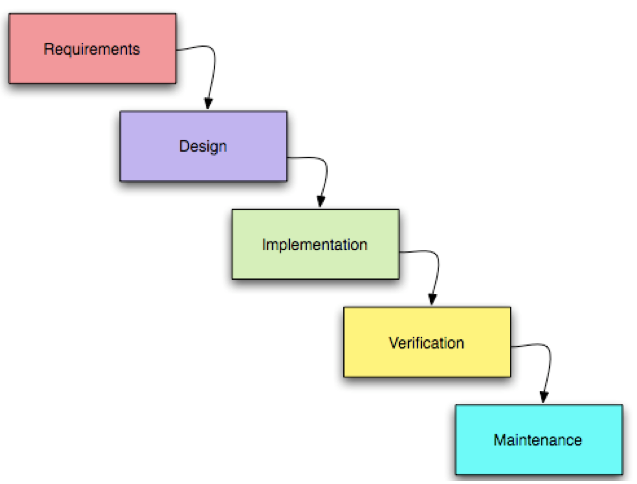
\includegraphics[width=8cm]{images/wasserfall_modell.png}
\end{minipage}

\subsection{V-Modell}
Grundidee: korrespondierende Tests \\
\begin{center}
	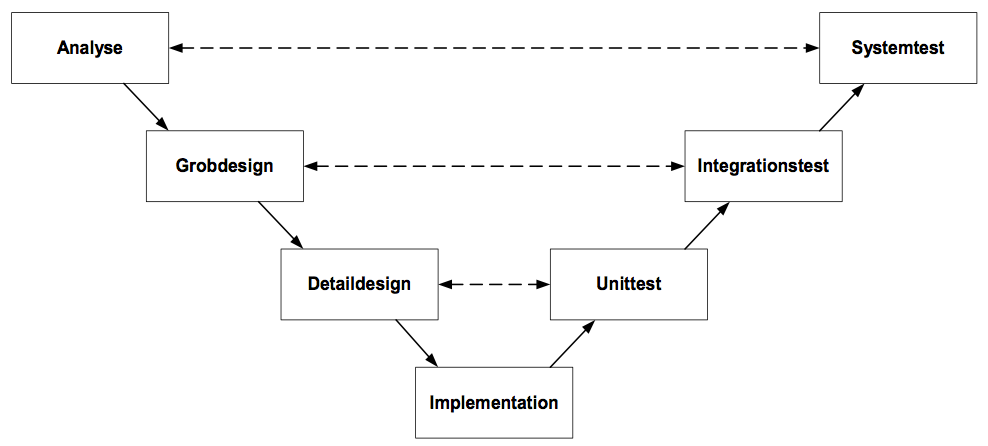
\includegraphics[width=12cm]{images/v_modell.png}
\end{center}

\subsection{Iterative / Inkrementelle Entwicklung}
\begin{minipage}{11cm}
	Grundidee: Software wird in einzelnen Schritten erstellt. \\
	
	\textbf{Inkrementell:}
		\begin{itemize}
			\item Resultat in Schritten entwickeln
			\item Jeder Schritt ist Teil des Endresultats
		\end{itemize}
	\textbf{Iterativ:}
		\begin{itemize}					
			\item Erste Version entwickeln
			\item In weiteren Schritten bessere Versionen erstellen
		\end{itemize}
\end{minipage}
\begin{minipage}{8cm}
	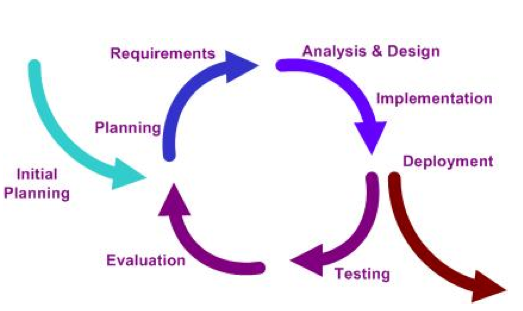
\includegraphics[width=8cm]{images/iterative_entwicklung.png}
\end{minipage}

\newpage %TODO: Newpage entfernen
\subsubsection{Spiralmodell}
Entwickelt von Barry Böhm, 1988
\begin{center}
	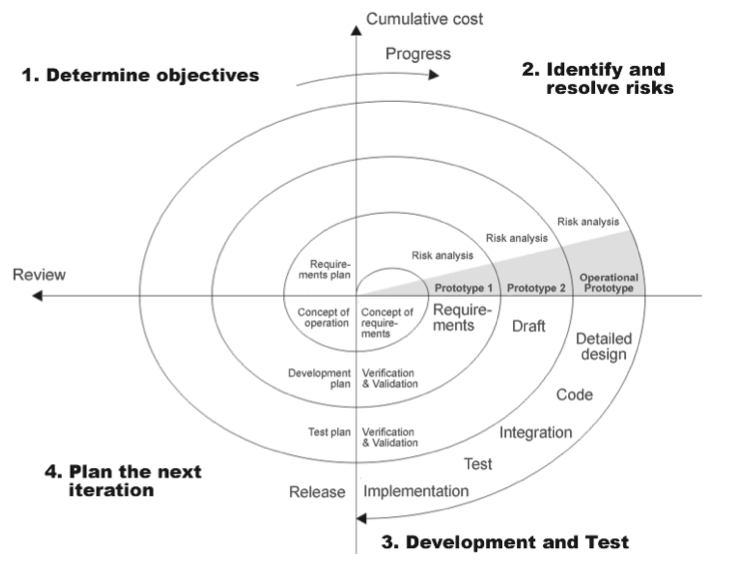
\includegraphics[width=12cm]{images/spiral_modell.png}
\end{center}

\subsection{Agile Softwareentwicklung}
\begin{itemize}
	\item Gegenbewegung zur herkömmlichen schwerfälligen, bürokratischen Softwareentwicklung
	\item agile = flink, beweglich
	\item Individuen und Interaktionen gelten mehr als Prozesse
	\item Grundlagen: Extreme Programming (Kent Beck, 1999); Agiles Mainfest (2001)
\end{itemize}

Agile Softwareentwicklung besteht aus:
\begin{enumerate}
	\item Agile \textit{Werte} bilden das Fundament.
	\item Agile \textit{Prinzipien} sind Handlungsgrundsätze, die auf agilen Werten basieren.
	\item Agile \textit{Methoden} sind konkrete Verfahren, die sich auf agile Werte und Prinzipien stützen.
	\item Agile \textit{Prozesse} sind die Zusammenfassung agiler Methoden. 
\end{enumerate}

\subsubsection{XP (Extreme Programming)}
\begin{minipage}{12cm}
	\begin{itemize}
		\item Bekanntester agiler Prozess
		\item Nach Buch ``Extreme Programming'' von Kent Beck (1999)
	\end{itemize}
\end{minipage}
\begin{minipage}{6cm}
	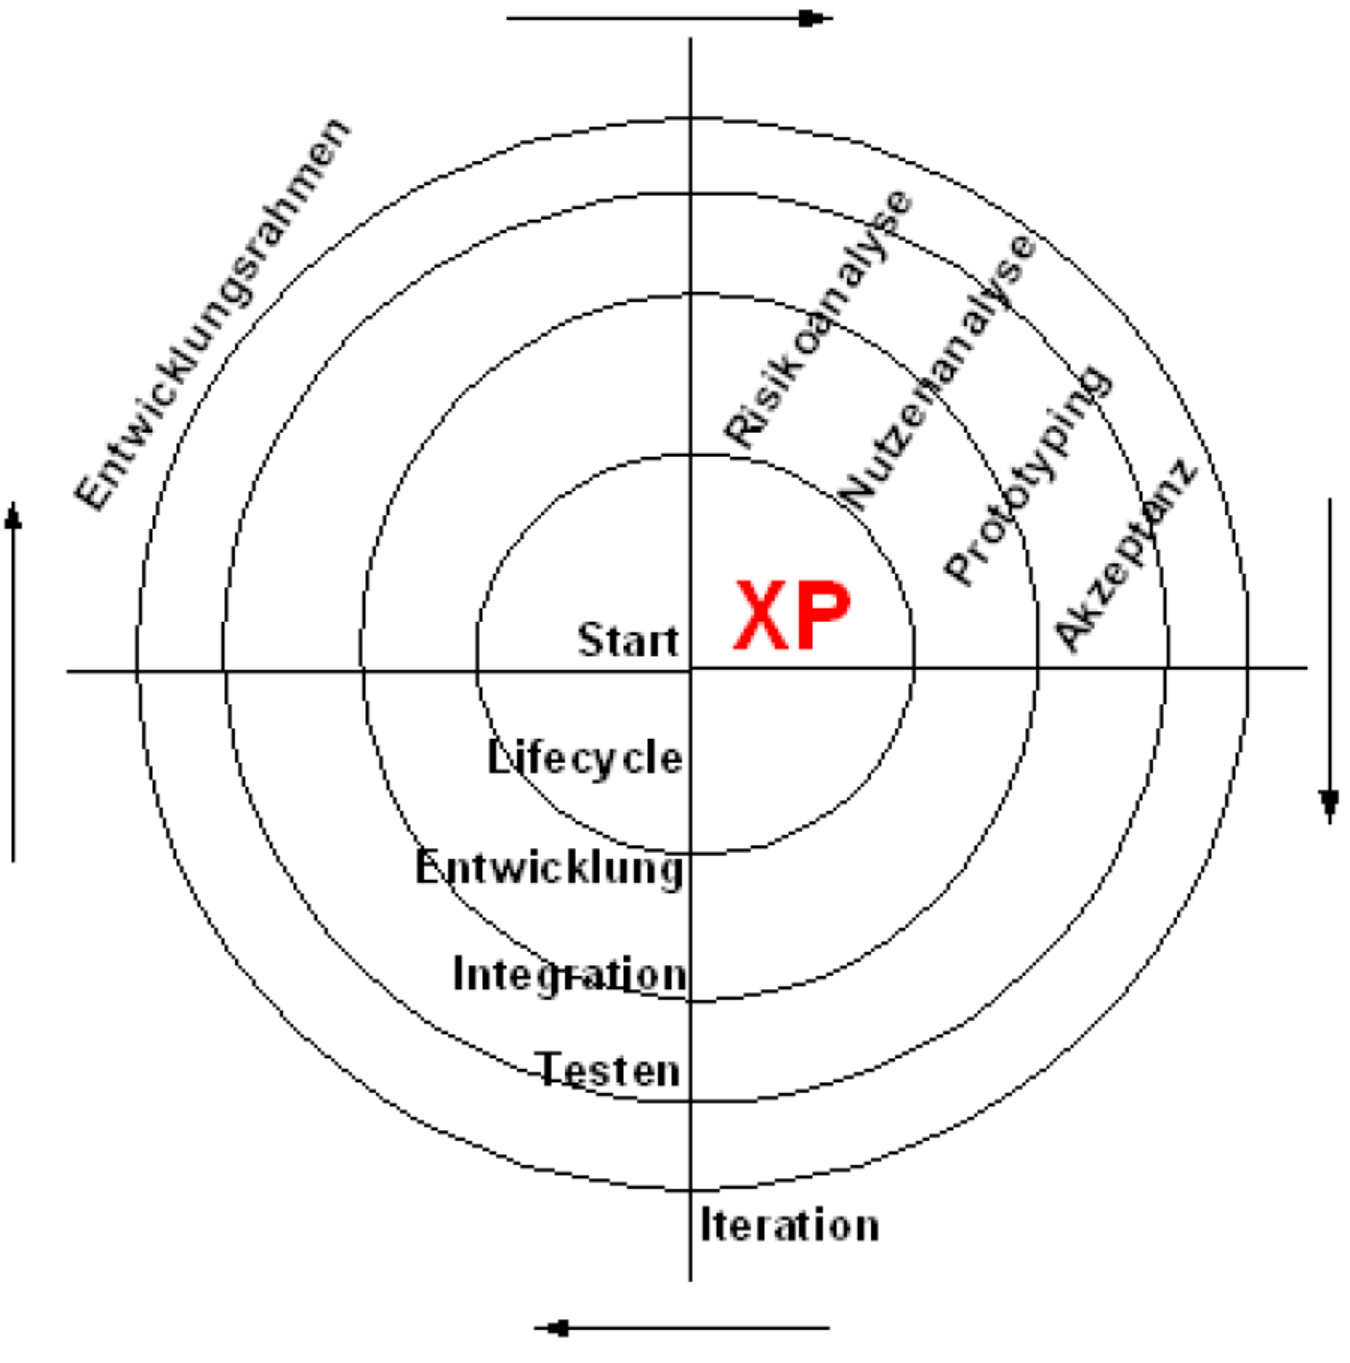
\includegraphics[width=6cm]{images/extreme_programming.png}
\end{minipage}

\subsubsection{Scrum}
\begin{minipage}{11cm}
	\begin{itemize}
		\item = ``Gedränge''
		\item Vorgestellt auf OOPSLA '95
		\item Basis: Sprints von 15-30 Tagen
	\end{itemize}
\end{minipage}
\begin{minipage}{8cm}
	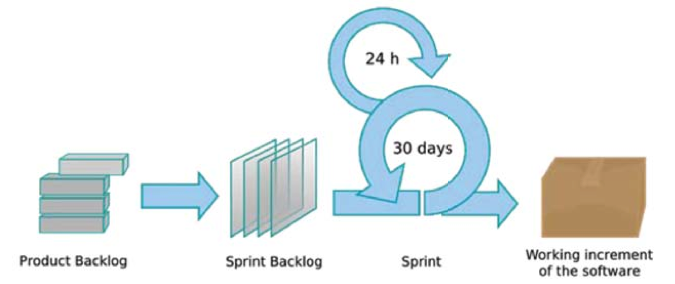
\includegraphics[width=8cm]{images/scrum.png}
\end{minipage}

\subsection{Objektorientierte Softwareentwicklung}
Grundidee: Modelle auf allen Stufen: OO-Analyse $\rightarrow$ OO-Design $\rightarrow$ OO-Implementation. Objekte entsprechen in der Regel realen Dingen; Änderungen werden daher weniger häufig und einfacher. \\

Kriterien für die Wahl des Modells:
\begin{itemize}
	\item Verfügbarkeit der Ressourcen
	\item Projektkomplexität
	\item Zeitpunkt von Änderungen (diskret, laufend)
	\item Qualität der Anforderungsdefinitionen
	\item Stabilität bzw. Volatilität der Anforderungen
\end{itemize}
\section{Testing}
\subsection{Allgemeine Begriffe}
\begin{itemize}
	\item \textbf{\textit{Definition:}} Programm mit der Absicht ausführen, Fehler zu finden. 
	\item Durch das Testen kann die Korrektheit eines Programms aber nicht bewiesen werden!
    \subitem Ausnahme: triviale Programme
	\item Mit Testen kann nur die Anwesenheit von Bugs bewiesen werden, aber nicht die Abwesenheit. 
	\item Erster Bug: 1947 wurde eine Motte im Relais eines Mark II Aiken Rechners entdeckt.
\end{itemize}
Nach sorgfältigem Testen steigt die Wahrscheinlichkeit, dass das Programm sich auch in nicht getesteten Fällen wunschgemäss verhält.
\begin{multicols}{2}
\subsubsection{Wahrscheinlichkeit von Fehlern}
Je mehr Fehler gefunden werden, desto höher ist die Wahrscheinlichkeit weiterer Fehler.\\
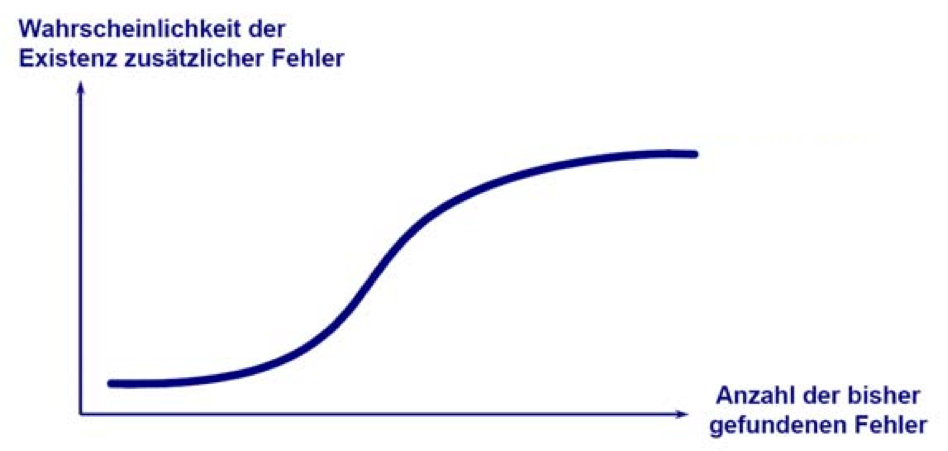
\includegraphics[width=6cm]{images/fehler_wkeit}
	
	\subsubsection{Testen \& Debuggen}
	\textbf{Ziel des Testing:} \\
	\begin{minipage}{10cm}
		\vspace{0.2cm}
		\begin{itemize}
			\item Aufzeigen, dass Fehler existieren.
			\item \textit{"{}Jeder gefundene Bug ist ein Gold Nugget"}
		\end{itemize}
		\textbf{Ziel des Debugging:} \\
		Durch Testing gefundene Fehler lokalisieren und beheben.		
	\end{minipage}
\end{multicols}

\begin{minipage}{10cm}
	\subsubsection{Verifikation \& Validierung}
	\textbf{Validierung:}\\
	\textit{"{}Are we building the right product?"}\\
	Überprüft das Produkt ob es die Anforderungen des Auftraggebers erfüllt.\\
	\textbf{Verifikation:}\\
	\textit{"{}Are we building the product right?"}\\
	Überprüft ob die erstellte Software funktioniert.\\
\end{minipage}
\begin{minipage}{7cm}
	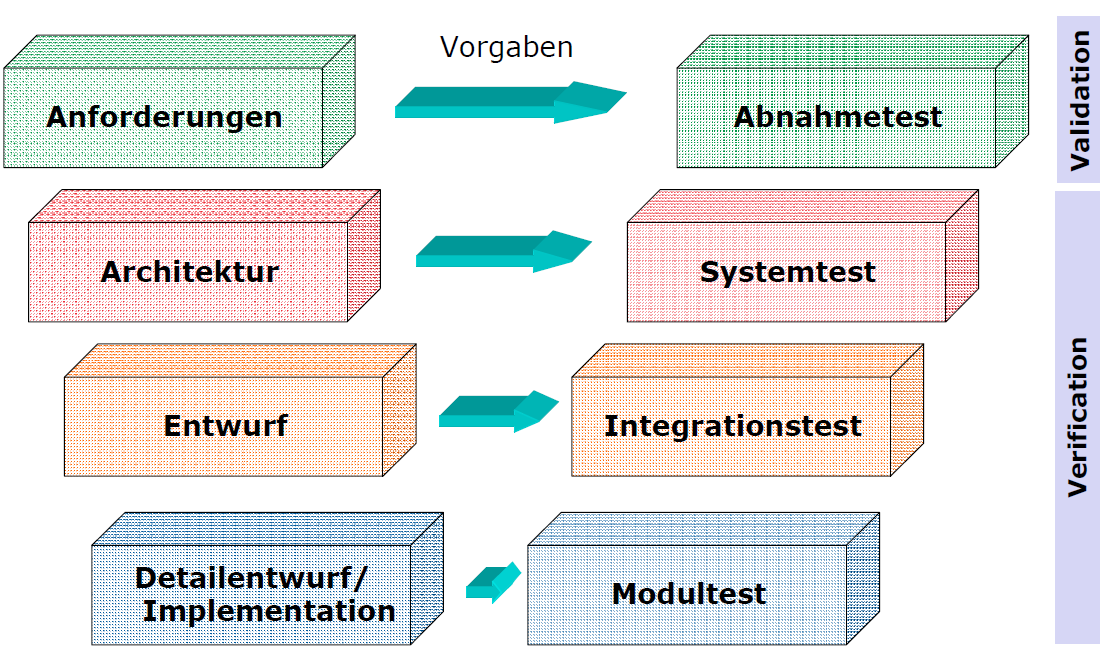
\includegraphics[width=7cm]{images/verificationvalidation}
\end{minipage}

\subsubsection{Anforderungen an Softwaretests}
	\begin{minipage}{10cm}
	\begin{itemize}
			\item Geplant: Testplanung $\rightarrow$ Testplan
			\item Systematisch spezifiziert $\rightarrow$ Testspezifikationen
			\item Testresultate festgehalten $\rightarrow$ Testprotokoll
			\item Reproduzierbarkeit:
			\begin{itemize}
				\item Wissen, was getestet wurde
				\item Unabhängig von testender Person
			\end{itemize}
			\item wenn möglich automatisiert
			\item Testspezifikationen laufend erweitern,\\
			$\Rightarrow$ Regressionstests
		\end{itemize}
	\end{minipage}
	\begin{minipage}{9cm}
		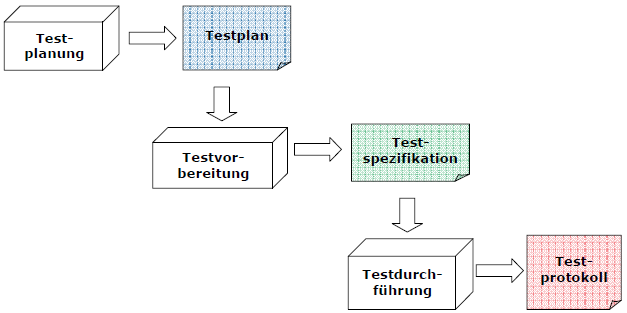
\includegraphics[width=\linewidth]{images/sofwaretest.png}
	\end{minipage}
\clearpage
\pagebreak

\begin{multicols}{2}
	\subsubsection{Massnahmen zur Softwareprüfung}
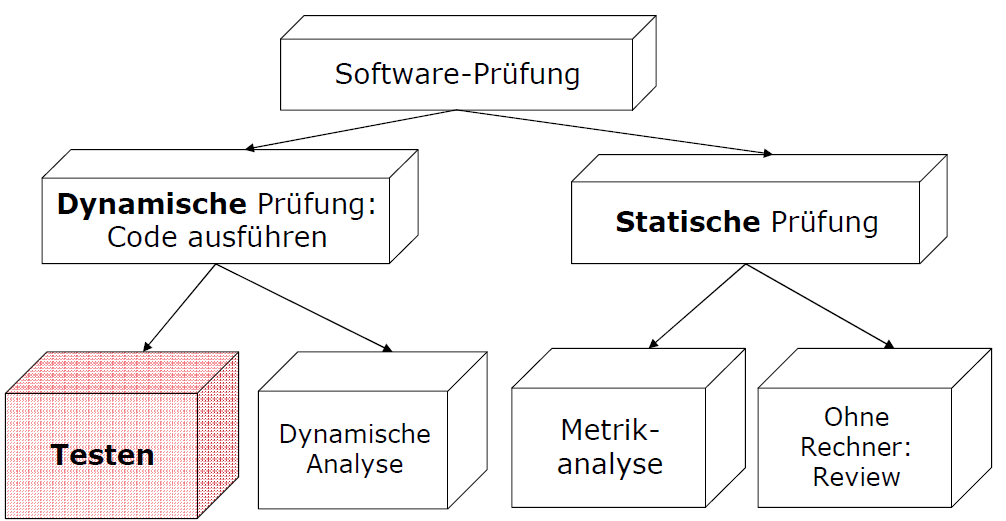
\includegraphics[width = 8cm]{images/massnahmenSoftwarepruefung}
	
	\subsubsection{Arten von Tests}
	\begin{minipage}{10cm}
\begin{tabular}{|p{5cm}|p{4cm}|}
	\hline
	\textbf{Anforderungskategorien} & \textbf{Testkategorien} \\ \hline
	\begin{itemize}
		\item Funktionale Anford.
		\item Nichtfunktionale Anford.
		\begin{itemize}
			\item Leistung
			\item Usability
		\end{itemize}
		\end{itemize} & 
		\begin{itemize}
		\item Funktionale Tests
		\item Nichtfunktionale Tests
		\begin{itemize}
			\item Leistungstests
			\item Usabilitytests
		\end{itemize}
	\end{itemize} \\ \hline
\end{tabular}
\end{minipage}
\end{multicols}

\subsection{Testmethoden}
\subsubsection{Testumgebung}
\begin{minipage}{0.5\linewidth}
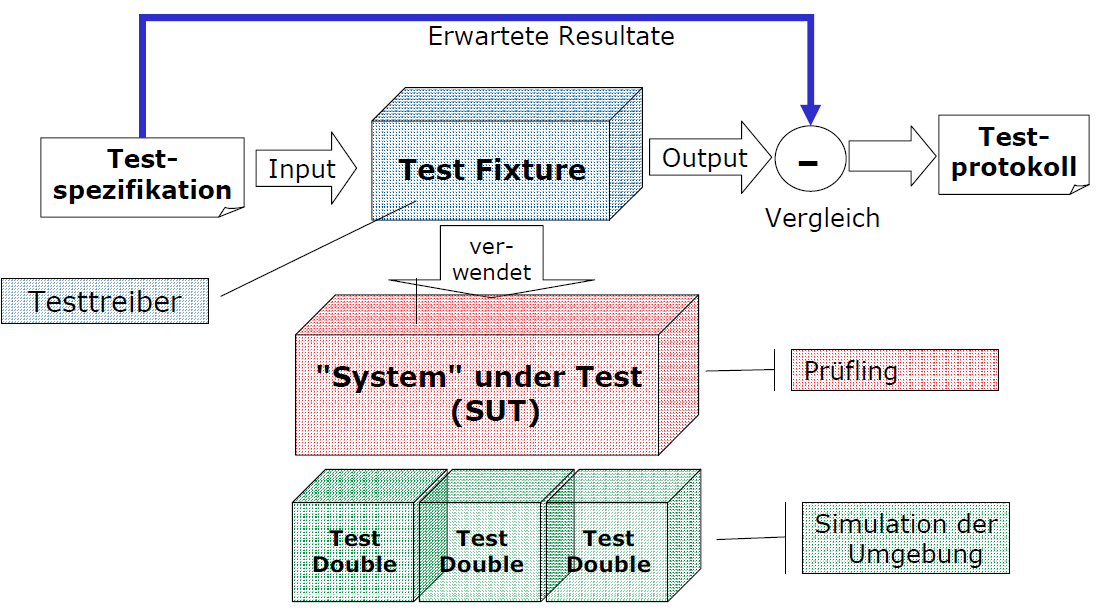
\includegraphics[width=\linewidth]{images/testumgebung}
\end{minipage}
\begin{minipage}{0.5\linewidth}
	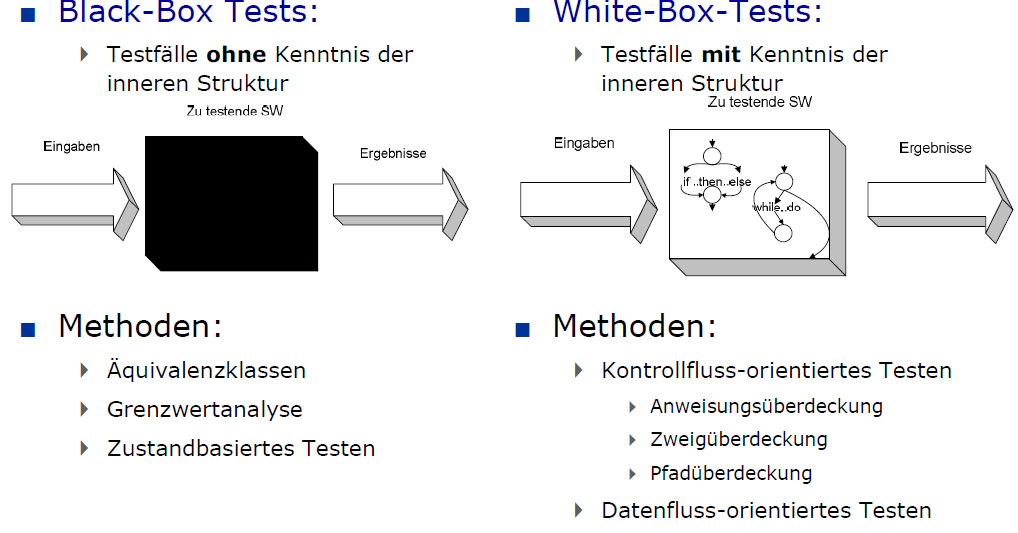
\includegraphics[width=\linewidth]{images/blackwhitetests}
\end{minipage}
\subsubsection{Blackbox Tests}
Testfälle \textbf{ohne} Kenntnis der inneren Struktur\\\\
\textbf{Äquivalenzklassen:} \\
\begin{minipage}{10cm}
Wertebereich, für welche das Programm voraussichtlich das gleiche Verhalten zeigt. \\
Methodik: 1 Testcase pro Äquivalenzklasse \\
Beispiel: Quadratische Gleichung; Determinante $<0$ ; $=0$ ; $>0$ \\
\vspace{2cm}
\end{minipage}
\begin{minipage}{5cm}
	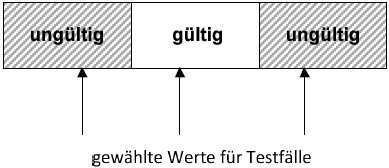
\includegraphics[width=\linewidth]{images/aequivalenzklasse.png}
\end{minipage}

\textbf{Grenzwertanalyse:} \\
\begin{minipage}{10cm}
Fehler liegen oft an Grenzen zulässiger Eingabewertbereiche. \\
\textit{\textbf{Methodik:}} Testfälle auf Grenzen und knapp daneben \\
\vspace{2cm}
\end{minipage}
\begin{minipage}{5cm}
	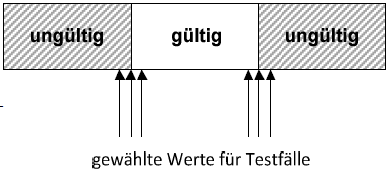
\includegraphics[width=\linewidth]{images/grenzwertanalyse.png}
\end{minipage}

\textbf{Zustandsbasiertes Testing:} \\
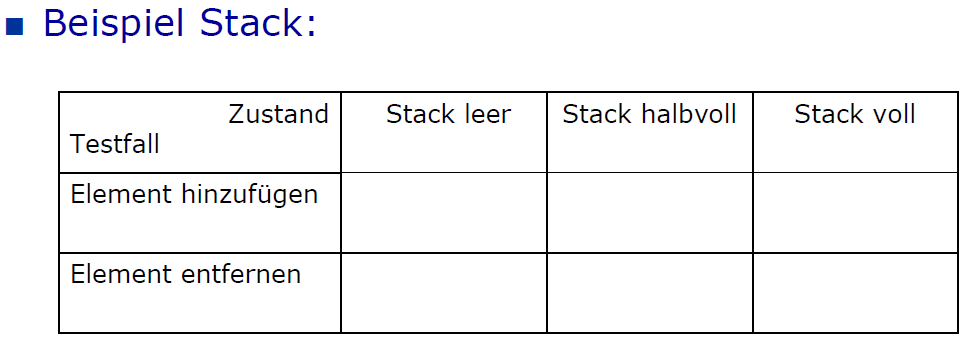
\includegraphics[width = 8cm]{images/stack}
\clearpage
\pagebreak
\subsubsection{Whitebox Tests}
\begin{minipage}{9cm}
    Tests \textbf{mit} Kenntnis der inneren Struktur\\
    
    \begin{itemize}
    \item Whitebox-Test werden mittels Kontrollfluss-Graphen durchgeführt.
    \begin{itemize}
    	\item Jedes Statement entspricht Knoten.
    	\item Zweige, stellen Schleifen und Verzweigungen dar, verbinden Knoten.
    \end{itemize}
    \item Der Test wird so ausgelegt, dass die Überdeckung (Coverage) möglichst gut ist. (Test der Überdeckung mit Dynamic Analyzer messen)
    \end{itemize}
\end{minipage}
\hspace{0.5cm}
\begin{minipage}{7.5cm}
	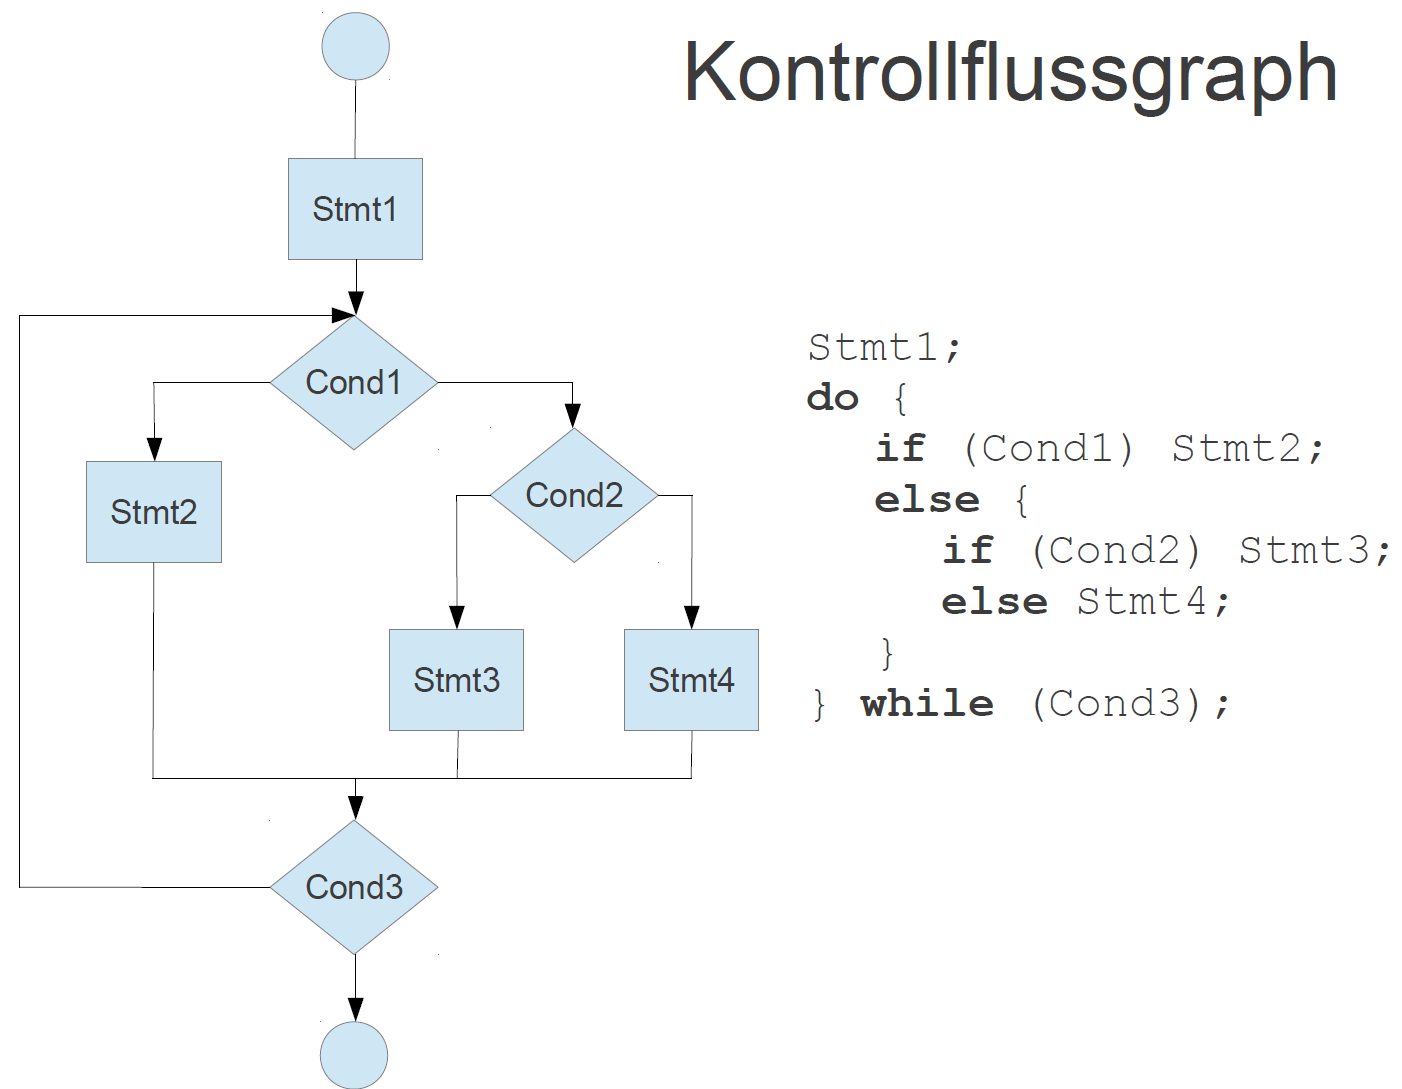
\includegraphics[width=\linewidth]{images/kontrollflussgraphen.png}
\end{minipage}

\paragraph{Testüberdeckung (test coverage)}
\begin{itemize}
	\item \textbf{\textit{Anweisungsüberdeckung (statement coverage)}}
			\begin{itemize}
				\item Prozentualer Anteil der Anweisungen welche im Test ausgeführt werden
				\item 100\% Anweisungsüberdeckung ist Minimum
			\end{itemize}
	\item \textbf{\textit{Zweigüberdeckung (branch coverage)}}
			\begin{itemize}
				\item Prozentualer Anteil der Zweige welche durchlaufen werden
				\item 100\% Zweigüberdeckung $\Rightarrow$ 100\% Anweisungsüberdeckung
			\end{itemize}
	\item \textbf{\textit{Bedingungsüberdeckung}}
			\begin{itemize}
				\item Verschiedene Kombinationen testen bei zusammengesetzten Bedingungen
				\item mind. 1x true/false durchlaufen
			\end{itemize}
	\item \textbf{\textit{Pfadüberdeckung (path coverage)}}
			\begin{itemize}
				\item Prozentualer Anteil der Pfade welche im Test durchlaufen werden
				\item Ein Pfad ist möglicher Weg durch Kontrollgraphen
			\end{itemize}
	\item \textbf{\textit{Funktionsüberdeckung}}
			\begin{itemize}
				\item \textit{"{}Tut es das, was der Kunde spezifiziert hat?"}
				\item 1 Szenario pro Use Case 
				\item Blackbox Tests
			\end{itemize}
\end{itemize}

\subsection{Testwerkzeuge}
\begin{minipage}{0.5\linewidth}
\begin{tabular}{ll}
	Blackbox: & FIT \\
	Whitebox: & xUnit
\end{tabular}
\\\\
	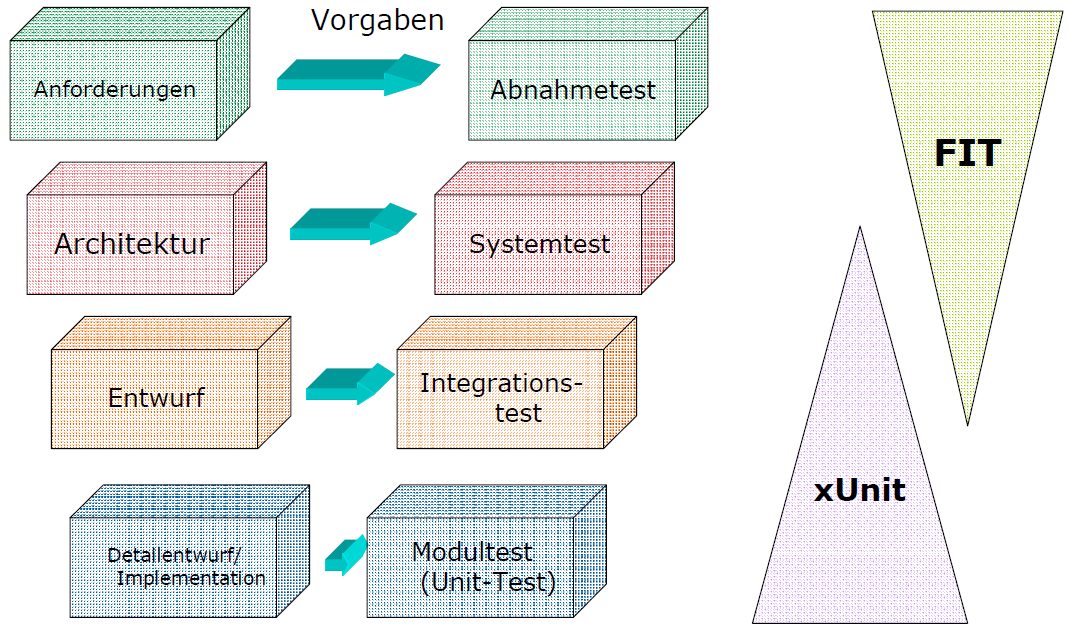
\includegraphics[width=\linewidth]{images/testwerkzeuge}
\end{minipage}
\begin{minipage}{0.5\linewidth}
	\subsection{Wer testet?}
	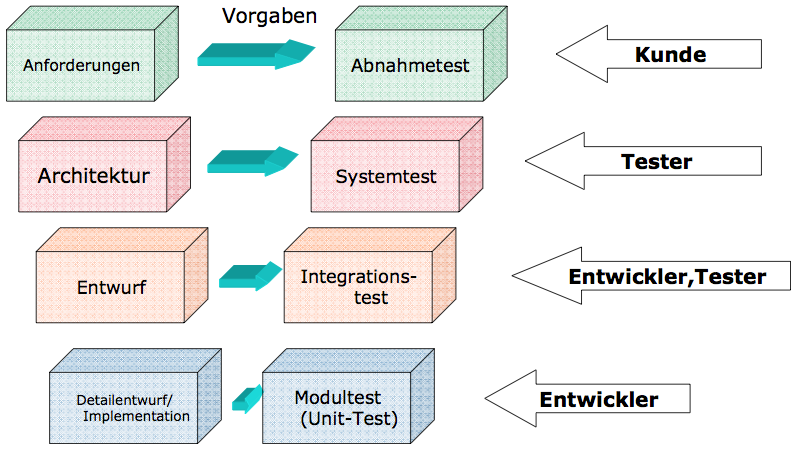
\includegraphics[width=\linewidth]{images/wer_testet}
\end{minipage}
\clearpage

\subsection{Automatisiertes Testing}
\textbf{\textcolor{mygreen}{Vorteile:}}
\begin{itemize}
	\item Wiederholbarkeit \newline $\Rightarrow$ Regressionstests möglich
	\item Eindeutige Spezifikationen (Testcode ist Programmcode)
\end{itemize}	
\textbf{\textcolor{red}{Nachteile:}}
\begin{itemize}
	\item Mehr Code zu schreiben und zu pflegen
	\item Testcode ist Programmcode: Wird überhaupt das Richtige getestet?
\end{itemize}

\subsection{Unit-Test}
\subsubsection{Konzept}
\begin{minipage}{10.5cm}
	\begin{itemize}
		\item Test häufig durch Programmierer selbst
		\item Test einer Komponente (Unit)
		\item Testen der Schnittstelle der Unit
		\item Im Voraus bekannte Ergebnisse $\rightarrow$ Assertions einfügen
		\item automatisch, wiederholbar
		\item heute mittels \textcolor{blue}{\textbf{Unit-Test-Frameworks}} \\
	\textbf{\textit{Frameworks:}} \textcolor{blue}{Programmgerüst} in welches das \textcolor{blue}{Anwendungsprogramm} eingebettet wird. Die Funktionen der Unit werden aus dem Framework heraus aufgerufen, sogenanntes \textbf{Hollywood-Prinzip:}\\\\
		\textit{"{}Don't call us, we'll call you"}
	\end{itemize}
\end{minipage}
\begin{minipage}{9cm}
	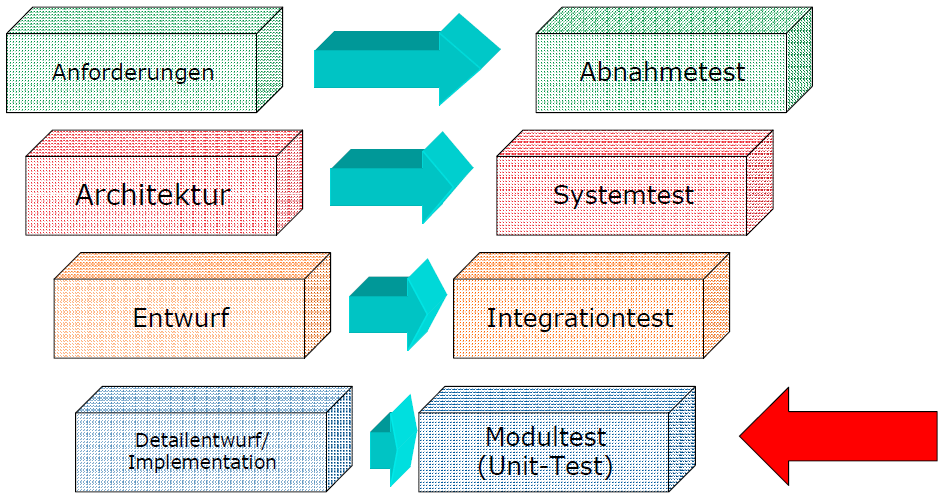
\includegraphics[width=9cm]{images/unittest}
\end{minipage}

\subsubsection{Arbeitsweise}
\begin{itemize}
	\item Spezielle, möglichst einfache Testfunktion mit Zusicherungen
	\begin{itemize}
		\item \texttt{ASSERT(...)} Vergleicht ein Soll- mit einem Ist-Wert
		\item Stimmen beide überein, ist der Test erfolgreich
		\item Sind sie unterschiedlich $\rightarrow$ Test fehlgeschlagen
	\end{itemize}
	\item Tests laufen automatisiert ab
	\item \textit{Test-Runner} = Programm, das die Test-Funktionen der Reihe nach ausführt
	\begin{itemize}
		\item Test-Run endet mit \"{}OK(...)\"{} oder \"{}FAILED: ...\"{}.
	\end{itemize}
	\item \textbf{Achtung: }
	\begin{itemize}
		\item \texttt{ASSERT(...)} - Anweisungen von Unit-Test nicht mit dem \"{}assert(...)\"{}-Makro aus \"{}assert.h\"{} verwechseln
	\end{itemize}
\end{itemize}

\subsubsection{Unit-Test Frameworks: Vorteile}
\begin{itemize}
	\item Übersichtliche Organisation der Testfälle
	\item Aufteilung der Tests auf mehrere Dateien in der Regel
	\begin{itemize}
		\item Zum Beispiel eine Testklasse pro zu testende Klasse.
	\end{itemize}
	\item Innerhalb der Datei: Organisation der Testfälle in Form von Testfunktionen und Testsuiten.
	\item Automatische Bereitstellung und Abbau einer Testumgebung ist möglich.
	\begin{itemize}
		\item bspw. \texttt{setUp(), tearDown()}
	\end{itemize}
	\item Testprotokolle: Ausgabe der Testergebnisse in verschiedenen Formen möglich. 
\end{itemize}
\begin{multicols}{2}
\subsubsection{CppUnit: Wichtige Begriffe}
\begin{minipage}{8cm}
	\footnotesize{
	\begin{itemize}
		\item \textcolor{blue}{Assert-Anweisung} \newline $\rightarrow$ Zum Vergleich von Ist- und Soll-Wert
		\item \textcolor{blue}{TestKlasse} \newline $\rightarrow$ selbst geschriebene Klasse, \newline
        welche von \"{}CppUnit::TestCase\"{} erbt.
		\item \textcolor{blue}{TestFunktion} \begin{itemize}
			\item enthält Assert-Anweisungen
			\item ist Memberfunktion einer Testklasse
		\end{itemize}
		\item \textcolor{blue}{TestSuite} \newline $\rightarrow$ zur Zusammenfassung von Testfunktionen
		\item \textcolor{blue}{TestFixture} \newline $\rightarrow$ zur Bereitstellung und Abbau einer Testumgebung
		\item \textcolor{blue}{Registry} \newline $\rightarrow$ zur Zusammenfassung von Testklassen
	\end{itemize}}
\end{minipage}
\subsubsection{CppUnit: Testklasse}
\hspace{0.5cm}
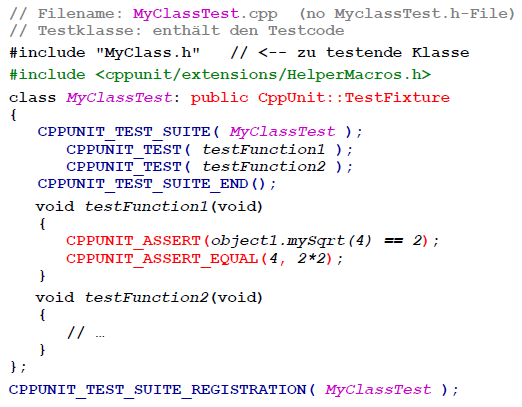
\includegraphics[width = 8cm]{images/testklasse}
\subsubsection{CppUnit: Konventionen}
\begin{itemize}
	\item Für jede zu testende Klasse wird eine entsprechende Testklasse erstellt
	\item Der Name einer Testklasse beginnt mit dem Namen der zu testenden Klasse und endet mit \"{}Test\"{}.
	\item Der Name einer Testfunktion beginnt mit \"{}test\"{}\newline Beispiel: \"{}testAddition()\"{}
\end{itemize} 
\subsubsection{Testprinzipien}
Erst der Test, dann der Code dazu
\subsubsection{Good Unit Tests are \"{}A TRIP\"{}}
\hspace{0.5cm}
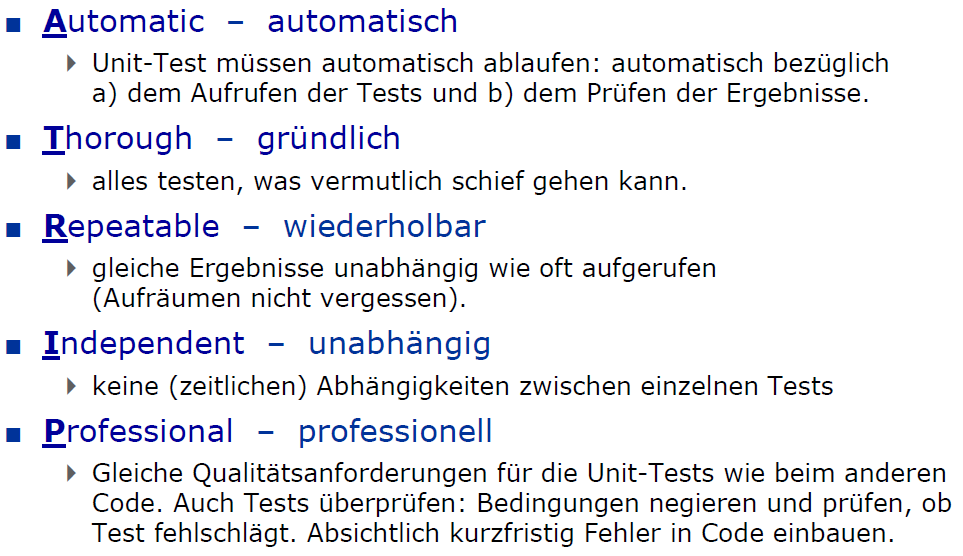
\includegraphics[width=8cm]{images/atrip}
\subsubsection{CORRECT - Boundary Conditions}
\hspace{0.5cm}
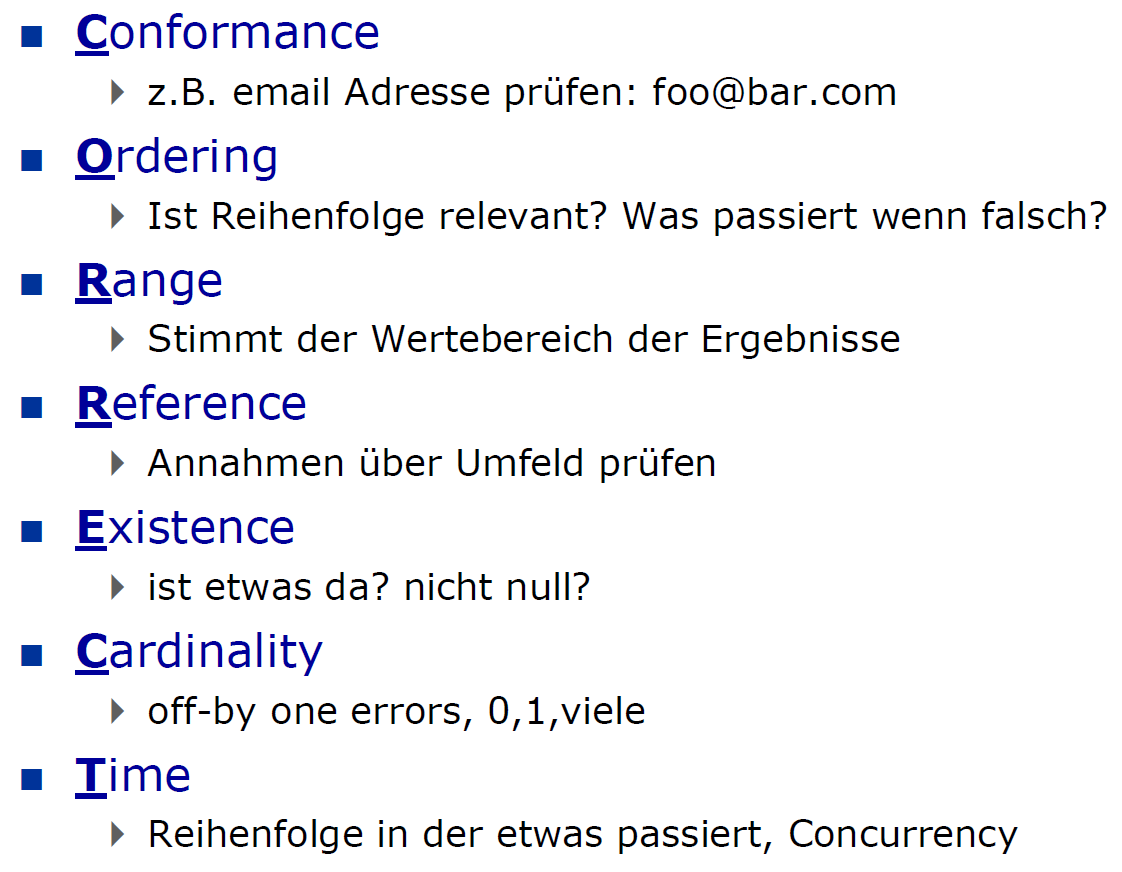
\includegraphics[width=6cm]{images/correct}
\subsubsection{CppUnit: Assert-Makros}
\begin{minipage}{10cm}
    \begin{itemize}
    \footnotesize{
    	\item \textcolor{blue}{\texttt{CPPUNIT\_ASSERT (condition)}}\newline 
    	\textcolor{blue}{\texttt{CPPUNIT\_ASSERT\_MESSAGE (msg, condition)}} \newline 
    	Test ist okay (d.h. wird bestanden), falls 'condition' true ist.
        
    	\item \textcolor{blue}{\texttt{CPPUNIT\_FAIL (msg)}} \newline
    	Test, der immer fehlschlägt.
        
    	\item \textcolor{blue}{\texttt{CPPUNIT\_ASSERT\_EQUAL (expected, actual)}} \newline 
    	\textcolor{blue}{\texttt{CPPUNIT\_ASSERT\_EQUAL\_MESSAGE (msg, expected, actual)}} \newline 
    	Test ist okay, falls 'expected' und 'actual' gleich sind. Dabei werden \newline einfache Datentypen ('int' etc.) sowie 'std::string' unterstützt.
        
    	\item \textcolor{blue}{\texttt{CPPUNIT\_ASSERT\_DOUBLES\_EQUAL (expected, actual, delta)}} \newline Test ist okay, falls 'expected' und 'actual' innerhalb einer Toleranz von \newline 'delta' gleich sind. Die Argumente sind vom Datentyp 'double'.
        
    	\item \textcolor{blue}{\texttt{CPPUNIT\_ASSERT\_THROW (expression, ExceptionType)}} \newline Test ist okay, falls 'expression' eine Ausnahme vom Typ 'ExceptionType' auslöst.
        
    	\item \textcolor{blue}{\texttt{CPPUNIT\_ASSERT\_NOTHROW (expression)}} \newline 
    	Test ist okay, falls 'expression' keine Ausnahme auslöst.
        
    	\item Bei den Varianten mit 'msg' (= message) wird diese zusätzlich \newline ausgegeben, falls der Test fehlschlägt.}
    \end{itemize}
\end{minipage}
\subsubsection{Typischer Output}
\hspace{0.5cm}
\begin{minipage}{10cm}
\footnotesize{
        \textbf{\textit{Suite hat 2 Tests fehlerlos absolviert}}\\
        ...\newline
        \textcolor{red}{\texttt{OK (2)}}\\\\
        
        \textbf{\textit{Suite hat 10 Tests mit Fehler in Test 2 und 5 absolviert}} \\ 
        ...\newline
        \textcolor{red}{\texttt{MyClassTest.cpp:32:Assertion \newline
        Test name: MyClassTest::testCtorWithValues\newline equality assertion failed\newline
        - Expected: 0 \newline - Actual : 15 \newline \newline        
        MyClassTest.cpp:57:Assertion\newline
        Test name: MyClassTest::testEquals\newline assertion failed\newline
        - Expression: object.isValid()\newline \newline        
        Failures !!!\newline
        Run: 10 \qquad Failure total: 2 \qquad Failures: 2 \qquad Errors: 0}}}
\end{minipage}
%\subsubsection{CppUnit Test-Fixture: \texttt{setUp()} und \texttt{tearDown()}}
%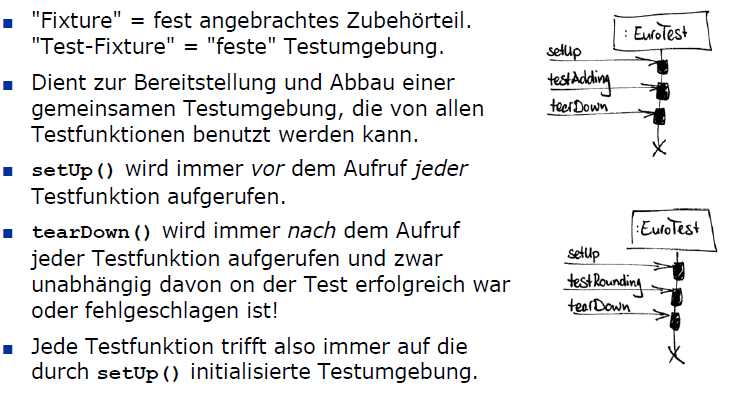
\includegraphics[width = 8 cm]{images/fixture}
\end{multicols}
\pagebreak
\section{Doxygen}
\pagebreak
\section{Projektmanagement}
\subsection{Grundlagen}

\subsubsection{Definition eines Projektes}
Ein Projekt ist ein zeitlich beschränktes Vorhaben zur Erzeugung eines einmaligen Produktes oder Dienstes. 

\subsubsection{Definition des Projektmanagement}
Das Projektmanagement bezeichnet die Gesamtheit von Führungsaufgaben, -organisation, -techniken und -mitteln für die Initiierung, Definition, Planung, Steuerung und den Abschluss von Projekten. 

\begin{multicols}{2}
	\subsubsection{Merkmale eines Projektes}
	\begin{itemize}
		\item einmaliges Vorhaben
		\item klare Ziele
		\item hat Risiken
		\item zeitlich begrenzt
		\item Kostenrahmen
		\item hat innovativen Charakter
		\item es arbeiten mehrere Personen daran
		\item hat Projektleiter \& Projektteam 
	\end{itemize} 
	
	\subsubsection{Kategorien von Projekten}
	\begin{itemize}
		\item Forschungs- und Entwicklungsprojekte
		\begin{itemize}
			\item  Entwicklung neuer Produkte
			\item  Erstellung von Software
		\end{itemize}			 
		\item Investitionsprojekte
		\begin{itemize}
			\item Bau eines Flughafen			
		\end{itemize}
		\item Organisationsprojekte
		\begin{itemize}
			\item Einführung Software
			\item Vorbereitung Veranstaltung
		\end{itemize}
	\end{itemize}
\end{multicols}

\subsubsection{Die 3 Eckpfeiler eines Projektes}
\begin{minipage}{10cm}
	Diese drei Grössen sind voneinander abhängig und sind auch bekannt als \textit{"Fast, Good, Cheap"}
	\begin{itemize}
		\item Ergebnis \textit{\"{}Scope\"{}} $\rightarrow$ Spezifikation
		\item Zeit \textit{"Time"} $\rightarrow$ Terminplan
		\item Aufwand \textit{"Cost"} $\rightarrow$ Budget
	\end{itemize}
\end{minipage}
\begin{minipage}{3cm}
	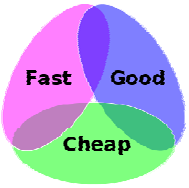
\includegraphics[width=3cm]{images/eckpfeiler.png}
\end{minipage}
\begin{minipage}{3cm}
	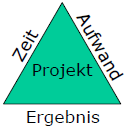
\includegraphics[width=3cm]{images/dreieck.png}
\end{minipage}

\subsubsection{Das Projektdreieck (Magisches Dreieck)}
\begin{minipage}{15cm}
	Diese drei Grössen werden als Dreieck dargestellt. Die Aufgabe des Projektmanagement ist es, ein sinnvolles Verhältnis dieser 3 herzustellen und während der Projektdauer zu gewährleisten. 
\end{minipage}

\subsubsection{Projektbeteiligten (Stakeholder)}
\begin{itemize}
	\item Auftraggeber $\rightarrow$ bezahlt \& befiehlt
	\item Projektleiter (PL) $\rightarrow$ Primär Manager, weniger Fachexperte
	\item Projektmitarbeiter (Projektteam) $\rightarrow$ Fachexperten, hohe Methoden und Sozialkompetenz
\end{itemize}

\subsubsection{Projektorganisationsformen}
\begin{multicols}{3}
	\begin{itemize}
		\item \textbf{Reine Projektorganisation}
		\begin{itemize}
			\item Projektleiter \& Projektteam arbeiten Vollzeit am Projekt
			\item Mitarbeiter sind voll\-kommen dem Projektleiter \newline unterstellt
			\item eher selten
		\end{itemize}
		\item \textbf{Matrix-Projektorganisation}
		\begin{itemize}
			\item Mitarbeiter aus spezif. \newline Bereichen arbeiten nur zeitweise am Projekt mit
			\item Verantwortung ist aufgeteilt zwischen Projektleiter/Linieninstanzen
			\item Häufigste Form
		\end{itemize}
		\item \textbf{Stabs-Projektorganisation}
		\begin{itemize}
			\item Hierarchie ist unverändert
			\item ergänzt durch Projektkoordinator hat keine \newline Weisungsbefugnisse
			\item stimmt Zusammenarbeit mit Mitarbeiter ab
		\end{itemize}
	\end{itemize}
\end{multicols}

\subsection{Projektablauf}
Jedes Projekt hat ein Anfang und ein Ende (Lebenszyklus). Der \textcolor{blue}{vorzeitige Abbruch} ist ein Unfall, ein sogenanntes \newline \textcolor{blue}{ungeplantes} Ende. Jedes Projekt besteht aus 4 Phasen. Die 4 Phasen überlappen sich und laufen parallel ab. \newline Während der Durchführung ist auch die Planung anzupassen. \\
\\
\begin{minipage}{8cm}
	\textbf{Projektphasen:}
	\begin{enumerate}
		\item Projektdefinition
        \subitem (Vorphase, Projektvorbereitung)
		\item Projektplanung
		\item Projektdurchführung
		\item Projektabschluss
	\end{enumerate}
\end{minipage}
\begin{minipage}{8cm}
	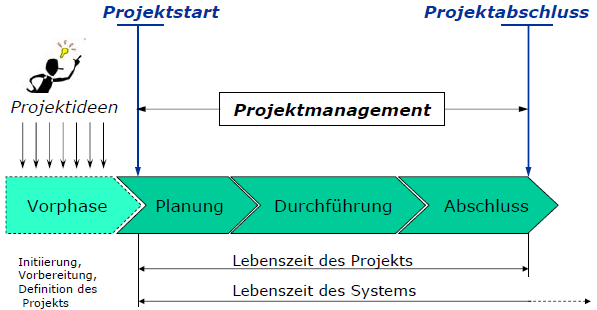
\includegraphics[width=\linewidth]{images/projektablauf.png}
\end{minipage}

\subsection{Projektphasen}
Verschiedene Teilprozesse können zeitlich parallel ablaufen. 
\subsubsection{Projektdefinition (Vorphase, Initiierung, Projektdefinition)}
\begin{itemize}
	\item Vorbereiten des Projektes
	\item evtl. Machbarkeitsstudie durchführen
	\item Ziele, Termine festlegen (Das Wichtigste eines Projektes)
	\item Grobe Aufwands- und Kostenschätzung, Projektorganisation festlegen
	\item Wird in formellen Projektauftrag festgehalten
\end{itemize}
	\begin{minipage}{9cm}
		\textbf{Projektauftrag} \\
		Der Projektauftrag ist ein schriftliches Dokument wo Ziele und Rahmenbedingungen festgehalten sind. Das Dokument wird vom Auftraggeber unterzeichnet, damit ist Existenz des Projektes formell bestätigt. \newline Die Ziele des Projektes sollten gemäss \textcolor{blue}{S.M.A.R.T.} formuliert sein.\newline
        {\small\textbf{ Häufige Bestandteile:}}
        \vspace{-0.3cm}
        \begin{multicols}{2}
            {\small
            \begin{itemize}
                \item Projektbezeichnung
                \item Auftraggeber
                \item Projektbeginn / -ende
                \item Kurzbeschreibung
                \item Projektergebnisse
                \item Projektbudget
                \item Projektleiter
                \item Terminvorgaben   
            \end{itemize}  }   
        \end{multicols}
	\end{minipage}
    \hfill
	\begin{minipage}{8.5cm}
		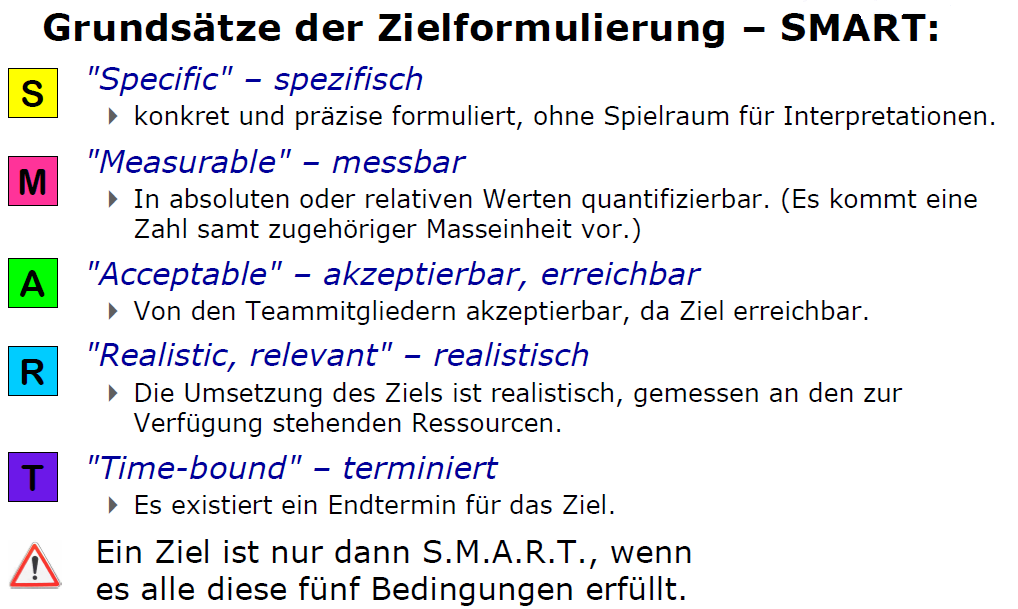
\includegraphics[width=\linewidth]{images/pmstart.png}
	\end{minipage}
\vspace{-0.5cm}	
\subsubsection{Projektplanung}
Als Voraussetzung zur Projektplanung gilt der erstellte Projektauftrag. Anschliessend findet das \textcolor{blue}{\textit{"Kick-Off-Meeting"}} statt. \newline Das \textit{"Kick-Off-Meeting"} gilt als \textcolor{blue}{offizieller Projektstart}., $\rightarrow$ \textbf{Hauptziel:} Alle sind arbeitsfähig!\\
Die Projektplanung ist das Wichtigste. Die Pläne werden periodisch überarbeitet da niemals alles nach Plan läuft. \newline 
$\rightarrow$ \textbf{Wichtig:} \textcolor{blue}{\textbf{Meilensteine}} setzen
\vspace{0.2cm}
\\
\begin{minipage}{10cm}
	\textbf{1. Projektstrukturplan (PSP)}
	\begin{itemize}
		\item Projekt in Teilprojekte zerlegen
		\item Kleinstmögliche Aufgaben sind Arbeitspakete
		\item Arbeitspakete sind \textcolor{blue}{phasenorientiert} (nach Zeitabschnitten) oder \textcolor{blue}{objektorientiert} (nach Komponenten) oder \textcolor{blue}{funktionsorientiert} (nach Ähnlichkeit der Aufgaben) aufgeteilt
		\item Pro Arbeitspaket wird eine Arbeitsbeschreibung erstellt
	\end{itemize} 	
\end{minipage}
\begin{minipage}{9cm}
	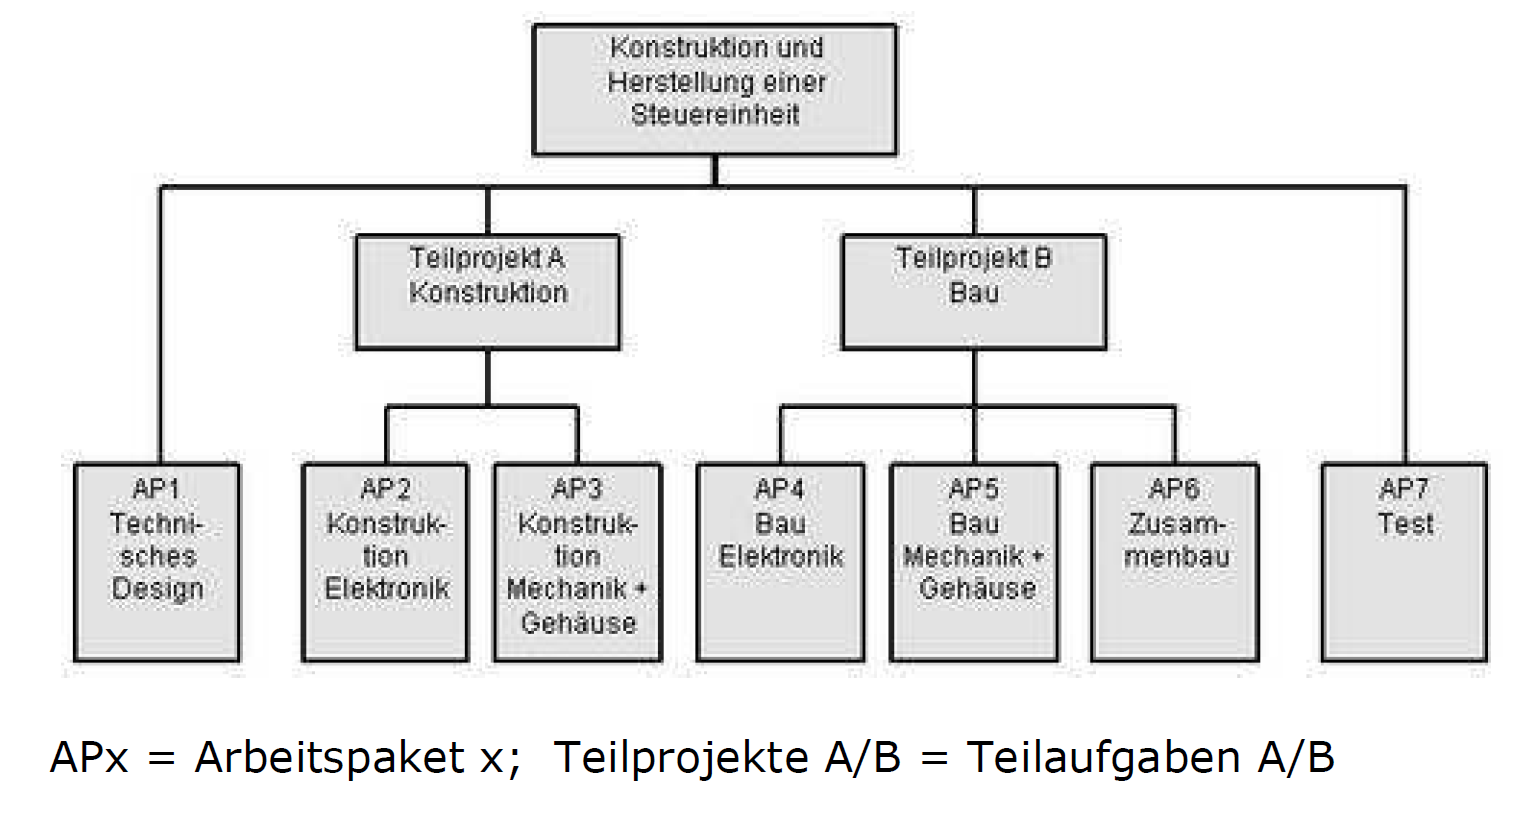
\includegraphics[width=9cm]{images/PSP.png}
\end{minipage}
\clearpage
\pagebreak

\textbf{Arbeitspakete}\\
\begin{center}
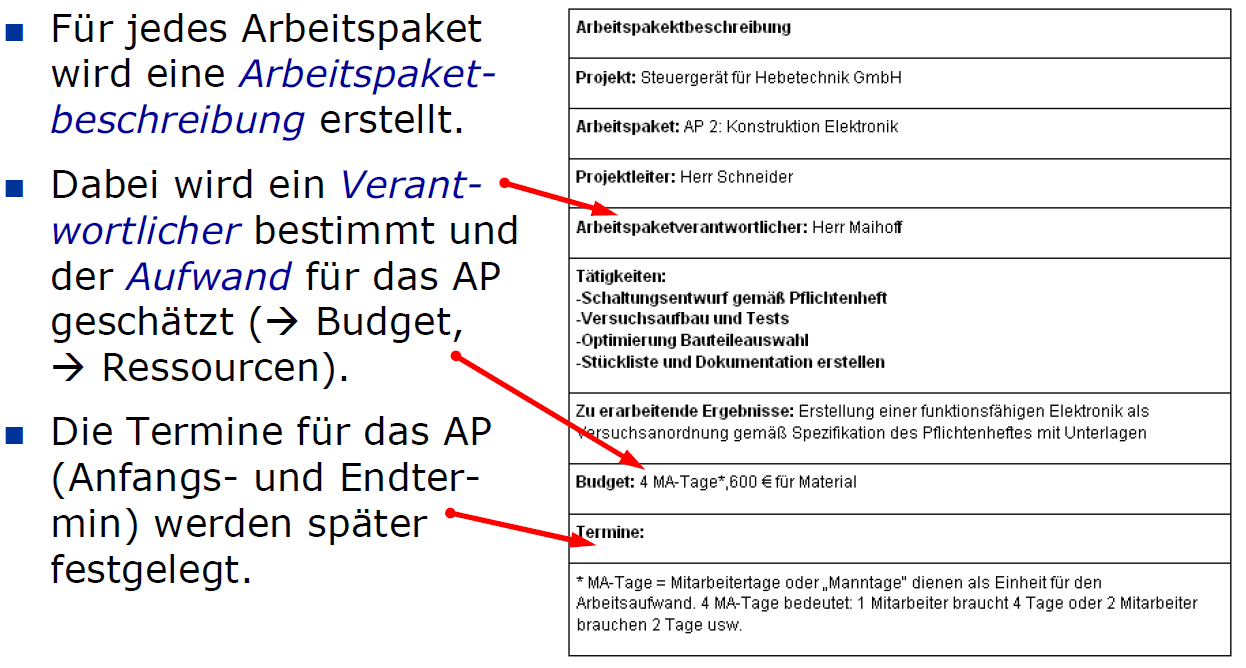
\includegraphics[width = 12cm]{images/arbeitsbeschreibung}
\end{center}
\vspace{-0.5cm}
\begin{multicols}{2}
\textbf{2. Projektablaufplan (PAP)} \\
Stellt die \textcolor{blue}{logische Abhängigkeiten} der Arbeitspakete dar. Dazu wird eine Vorgangsliste erstellt, welche die Abhängigkeiten zwischen den Arbeitspakete aufzeigt. \\
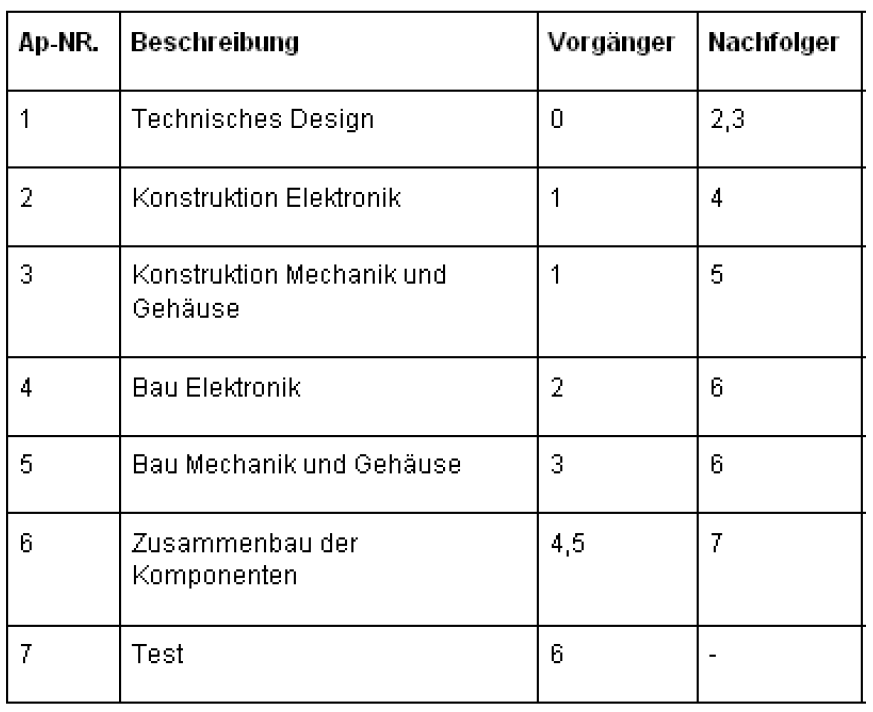
\includegraphics[width = 6cm]{images/ablaufsplan}
\end{multicols}

\renewcommand{\arraystretch}{1.2}
	\begin{tabular}{|l|l|l|}
		\hline \textbf{Abhängigkeit} & \textbf{Funktion} & \textbf{Bild} \\
		\hline Normalfolge & Nachfolger kann erst beginnen, wenn Vorgänger beendet ist & \tabbild[width=4cm]{images/normalfolge.png}\\
		\hline Anfangsfolge & Nachfolger kann erst beginnen, wenn Vorgänger begonnen hat &
		\tabbild[width=4cm]{images/anfangsfolge} \\
		\hline Endfolge & Nachfolger kann erst enden, wenn Vorgänger beendet ist &
		\tabbild[width=4cm]{images/endfolge.png} \\
		\hline Sprungfolge & Nachfolger kann erst enden wenn Vorgänger begonnen hat &
		\tabbild[width=4cm]{images/sprungfolge.png}\\
		\hline
	\end{tabular}\newline
\vspace{0.2cm}
\\
\\
\textbf{3. Projektterminplan}
\begin{itemize}
	\item Zuordnung von Terminen zu den Arbeitspaketen
	\item Festlegen der \textcolor{blue}{Meilensteine/Milestones} (= wichtige Termine)
    \begin{itemize}
    	\item Meilensteine sind Etappenziele welche zur Projektkontrolle dienen
    	\item Meilensteine sind so formuliert, dass \textit{"'Erfüllt"} oder \textit{" Nicht Erfüllt"} gilt
    	\item Meilensteine stehen am Ende jeder Projektphase    	
    \end{itemize}
	\item Projektterminplan wird aufgrund des PSP und PAP erstellt
\end{itemize}
	\begin{tabular}{l l l}
		 \textbf{Balkendiagramm} & \textbf{Netzplan} & \textbf{Microsoft Project} \\
		 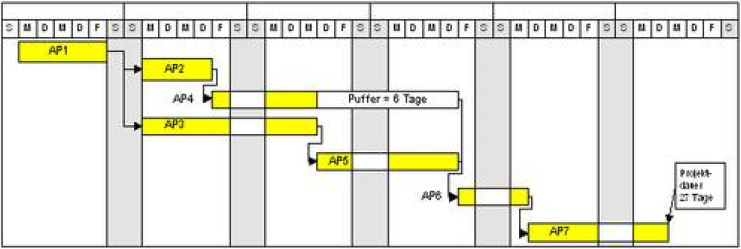
\includegraphics[width=6cm]{images/balkendiagramm} & 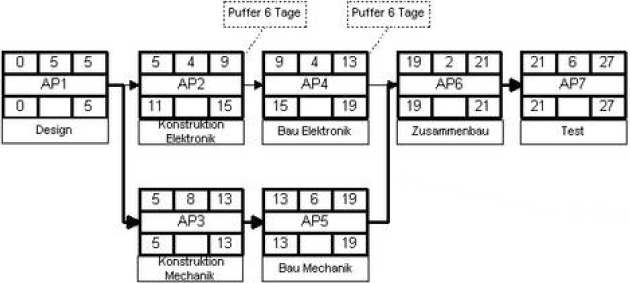
\includegraphics[width=6cm]{images/netzplan}	& 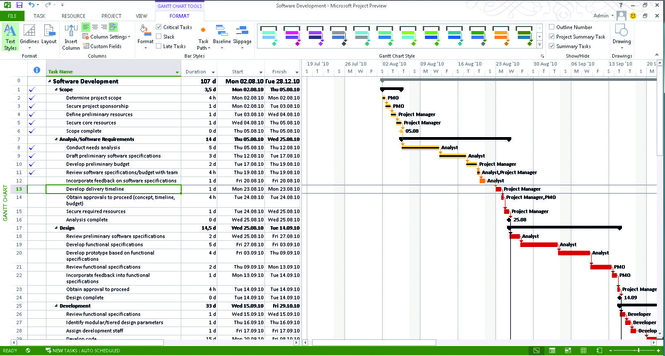
\includegraphics[width=6cm]{images/msproject}	 
	\end{tabular}
\clearpage

\textbf{3.1 Microsoft Project}\\
In MS Project wird immer von Task (Vorgang) gesprochen.\newline
MS Project hat als Grundlage das Balkendiagramm und die Netzplantechnik.\\
Wichtigster Zusammenhang: \textbf{Work = Duration $\cdot$ Units}\\
\begin{multicols}{2}
	\begin{itemize}
		\item \textbf{Einzelvorgang (Sub Task)} $\rightarrow$ Arbeitspaket
		\item \textbf{Sammelvorgang (Summary Task)} \newline $\rightarrow$ mehrere Vorgänge
		\item \textbf{Vorgang mit Dauer 0} $\rightarrow$ Meilenstein	
	\end{itemize}
	\begin{itemize}
		\item \textbf{Fixed Units} $\rightarrow$ Ressourcen = konstant
		\item \textbf{Fixed Work} $\rightarrow$ Arbeit = konstant
		\item \textbf{Fixed Duration} $\rightarrow$ Dauer = konstant
	\end{itemize}
\end{multicols}

\begin{tabular}{|l|l|l|}
	\hline \textbf{Work}& Arbeitsumfang & Einheit: Anzahl Personentage, Mannstunden\\
	\hline \textbf{Duration} & Zeitdauer & Einheit: Anzahl Stunden,Tage\\
	\hline \textbf{Units}& Intensität& Einheit: Angabe der Beteiligung in Prozent\\
	\hline
\end{tabular}\\\\
\textbf{4. Ressourcen- und Kapazitätsplan}\\
Die benötigten Ressourcen ermitteln und mit den Kapazitäten abstimmen. 
\\
\\
\textbf{5. Kosten- und Budgetplan}\\
Die Kosten für für die Ressourcen schätzen und Budget erstellen. 

\subsubsection{Projektdurchführung}
Die eigentliche Arbeit beginnt. Der Projektleiter hat die Aufgabe des Projekt-Controlling (to control $\rightarrow$ steuern).\\
\textcolor{blue}{Projekt-Controlling = Projektkontrolle + Projektsteuerung}
\renewcommand{\arraystretch}{1.2}
\begin{table}[h!]
	\begin{tabular}{|l|l|}
		\hline \textbf{Projektkontrolle} 	& Rechtzeitiges Feststellen von Abweichungen gegenüber dem geplanten \\ 
		& Soll-Ist-Vergleich\\
		\hline  \textbf{Projektsteuerung} 	& Massnahmen um Projekt bei Abweichungen wieder auf Zielkurs zu bringen. \\
		& Soll-Werte anpassen\\
		\hline
	\end{tabular}
\end{table}

\subsubsection{Projektabschluss}
\begin{itemize}
	\item Eigentliche Projektarbeit wurde erfolgreich abgeschlossen.
	\begin{itemize}
		\item Ziele sind erreicht
	\end{itemize}
	\item Formaler Abschluss des Projekts mit dem Auftraggeber:
	\begin{itemize}
		\item Projektpräsentation
		\item Projektabnahme, Übergabe, Entlastung des PL.
		\item Allfällige Nacharbeiten
	\end{itemize}
	\item Projektteam interner Abschluss
	\begin{itemize}
		\item Abschlussmeeting: Manöverkritik, \"{}Lessons learned\"{}
		\item Abschlussfeier
	\end{itemize}
\end{itemize}
\clearpage
\section{Versionskontrolle}
\subsection{Versionskontrollsysteme (VCS)}

\begin{multicols}{2}
	\subsubsection{Zweck}
	\begin{itemize}
		\item Aufbewahrung, Verwaltung, Wiederherstellen von früheren Versionen in einem Archiv
		\item Koordination des Zugriffs, bekannt als File-Sharing
		\item erlaubt hervorholen von alten Versionen
	\end{itemize}
	
	\subsubsection{Haupteinsatz}
	\begin{itemize}
		\item Softwareentwicklung: zur Verwaltung des Source-Codes
		\item Dokument-Management-Systeme (DMS)
		\item Archiv $=$ Repository $=$ Lager
	\end{itemize}
\end{multicols}

\subsubsection{Hauptaufgaben von VCS}
\begin{minipage}{\linewidth}
	\begin{itemize}
		\item \textcolor{blue}{Protokollierungen} der Änderungen: \newline $\rightarrow$ Es kann jederzeit nachvollzogen werden, wer wann was geändert hat.
		\item \textcolor{blue}{Wiederherstellung} von alten Ständen (Milestones) einzelner Dateien: \newline $\rightarrow$ Versehentliche Änderungen können jederzeit rückgängig gemacht werden.
		\item \textcolor{blue}{Koordinierung} des gemeinsamen Zugriffs auf die Dateien eines Projektes. \newline $\rightarrow$ Mehrere Mitarbeiter können gefahrlos auf die Dateien eines Projektes zugreifen. 
		\item \textcolor{blue}{Mehrere Entwicklungszweige} (engl. \"{}Branches\"{})\newline $\rightarrow$ Es kann gleichzeitig an verschiedenen Entwicklungszweigen gearbeitet werden. \newline $\rightarrow$ Ein \"{}Branch\"{} ist eine Abspaltung von der normalen Entwicklungslinie, bei der z.B. eine alternative Lösung für ein Teilproblem untersucht wird.
	\end{itemize}
\end{minipage}
\subsubsection{Einteilung von VCS}
	\begin{itemize}
\item \textcolor{blue}{Lokale (dateibasierte) Versions-Kontrollsysteme}
\begin{itemize}
\item \"{}Local Version Contol System\"{} (LVCS)
 \item Dateibasiert = \textbf{ein} Archiv für \textbf{jede} zu archivierende Datei
 \item Der Name der Archiv-Datei wird dabei vom Namen des Source-Files abgeleitet. \newline $\rightarrow$ \texttt{hallo.cpp} $\rightarrow$ \texttt{hallo.cpp\textbf{,v}} (Suffix '\textbf{,v}') 
 \item Die im Archiv \"{}abc.xyz,v\"{} abgespeicherte Versionen der Datei \"{}abc.xyz\"{} werden \"{}Revisionen\"{} genannt.
 \item Wichtige Operationen:
 \begin{itemize}
 	\item \textbf{\"{}check-in\"{}:} Datei zu Archiv hinzufügen (neue Revision) \newline $\rightarrow$ \texttt{\$ ci -m \"{}first check-in\"{} hallo.cpp \qquad \# \"{}einchecken\"{}}
 	\item \textbf{\"{}checkout\"{}:} eine bestimmte Revision aus dem Archiv holen \newline $\rightarrow$ \texttt{\$ co -l hallo.cpp\qquad \# \"{}auschecken\"{} und \"{}locken\"{}}
 \end{itemize}
\end{itemize}
\item \textcolor{blue}{Zentralisierte Versions-Kontrollsysteme}
\begin{itemize}
	\item \"{}Centralized Version Control Systems\"{} (CVCS)
	\item \textbf{\textit{Ein}} zentrales Archiv für alle zu archivierende Dateien. 
\end{itemize}
\item \textcolor{blue}{Verteilte Versions-Kontrollsysteme}
\begin{itemize}
	\item \"{}Distributed Version Control Systems\"{} (DVCS)
	\item \textbf{\textit{Mehrere, verteilte, gleichberechtigte}} Archive für die zu archivierenden Dateien
	\item \textbf{Git}, gehört in diese Sparte!
\end{itemize}
\end{itemize}
\clearpage
\subsection{Git}
\begin{itemize}
	\item Git $\rightarrow$ (engl. Blödmann)
	\item Entwickelt von Linus Torvalds, Linux-Erfinder
	\item Ziele waren Geschwindigkeit, Einfachheit, Unterstützung von nichtlinearer Entwicklung, \newline vollständig verteilt (distributed Repos), Verwaltung von grossen Projekten
	\item Ist ein spezielles Filesystem
	\item Git ist ein DVCS
\end{itemize}

\subsubsection{Allgemeines}
\begin{tabular}{|l|l|}
	\hline \textbf{Repository} &
    Ist ein Archiv für ein Projekt und enthält alle Änderungen und Versionen
    \\ 	\hline     
    \textbf{Branch} &
    Beschreibt zusammenhängende Änderungen in einem Projekt. Es gibt Minimum einen  bis beliebig viele.
    \\
    &
    Der Master-Branch ist der Produktivzweig
    \\ \hline
    \textbf{Commit} &
    Beschreibt eine Änderung in einem Branch an einer Datei mit Änderungsinformation
    \\ \hline
    \textbf{Snapshot} &
    Momentanes Zeitabbild des Projektes
    \\ \hline
    \textbf{Merge} &
    Zusammenführen von Änderungen aus zwei Branches
    \\	\hline
    \textbf{Stagen} &
    Datei zum Index hinzufügen
    \\\hline
\end{tabular}
\\
\\
\begin{tabular}{|c|c|}
	\hline \textbf{Lifecycle von Dateien} & \textbf{Branch}\\
	\hline \tabbild[width=9cm]{images/git_lifecycle.png} & \tabbild[width=9cm]{images/git_branch.png}\\
	\hline
\end{tabular}

\subsubsection{Git-Konzepte}
\begin{itemize}
	\item Git-Workspace ist ein Verzeichnis welches die zu bearbeitenden Dateien eines Projektes enthält
	\item In diesem Verzeichnis ist ein Unterverzeichnis \textit{".git"}
	\item Dieses Unterverzeichnis \textit{".git"} bildet das lokale Repository
	\item Im Branch zeigen die Pointer immer auf den vorhergehenden Commit
\end{itemize}

\subsubsection{Datenbereiche}
\begin{tabular}{|l|l|}
	\hline
	\begin{tabular}[c]{@{}l@{}}\textbf{Workspace}\\ -Projektverzeichniss\\ -enthält die Dateien mit denen man arbeitet\end{tabular}   & \begin{tabular}[c]{@{}l@{}}\textbf{Repository}\\ -enthält die Versionsgeschichte in Form von Commits (Revision)\\ -lokal/remote\end{tabular}   \\ \hline
	\begin{tabular}[c]{@{}l@{}}\textbf{Stash}\\ -Lager\\ -zum temporären Speichern der Workspace-Daten\end{tabular} & \begin{tabular}[c]{@{}l@{}}\textbf{Staging Area/Index/Cache}\\ -sammelt Änderungen für Commits\\ -Bereitstellungsraum\end{tabular} \\ \hline
\end{tabular}
\\
	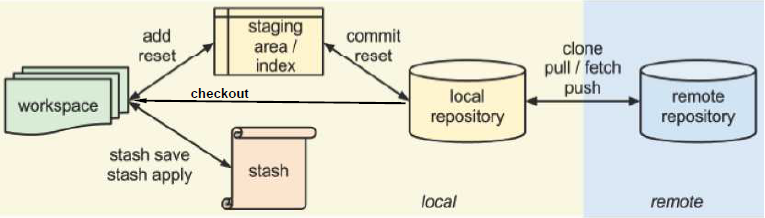
\includegraphics[width=12cm]{images/git.png}

\subsubsection{Git-Repository}
\begin{itemize}
	\item \textbf{lokales Repository} $\rightarrow$ \textit{".git"}-Verzeichniss im Workspace
	\item \textbf{remote Repository} $\rightarrow$ Ein normales Git-Repository ohne Projektverzeichnis an externem Ort
	\item \textbf{\"{}bare\"{} Repository} $\rightarrow$ Git-Repository ohne Projektverzeichnis zum teilen, Klon von lokalen Repositories
\end{itemize}
\subsubsection{Git-Hashwerte}
\begin{itemize}
	\item Zur Identifizierung von Commits (und anderen Git-Objekten) werden sogenannte Hash-Werte verwendet
	\item Diese werden mittels SHA1-Algorithmus berechnet.\newline $\rightarrow$ SHA-1 = \"{}Secure Hash Algorithmus Version 1\"{}\newline
	$\rightarrow$ Dieser liefert 160 Bits (40 Hex Ziffern), \textbf{eindeutiger Prüfwert} für beliebige Daten
	\item die Hash-Werte werden als Zweigerwerte (Adressen) verwendet um die Repository-Datenstruktur aufzubauen
	\item Der Hashwert wird aus dem Dateiinhalt berechnet und für den Dateinamen verwendet
\end{itemize}
\subsubsection{Ein existierendes Verzeichnis als Repository initialisieren}
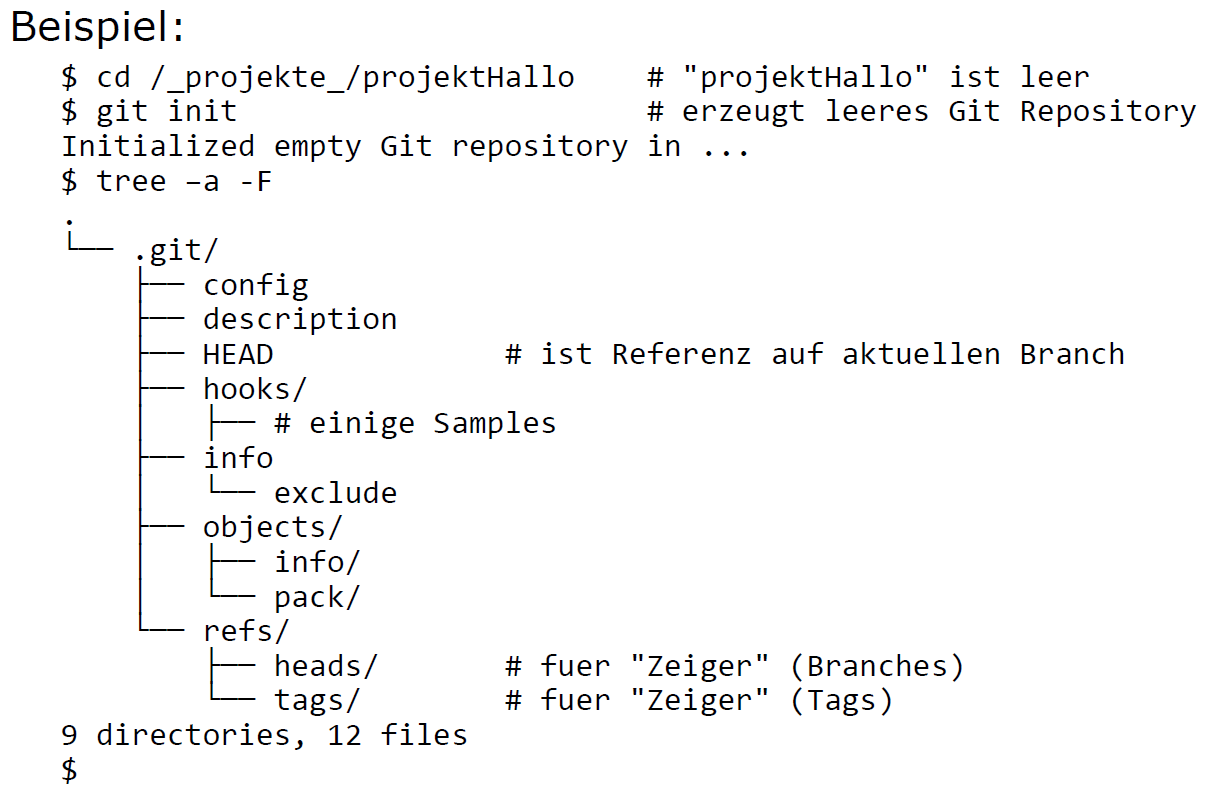
\includegraphics[width = 13cm]{images/bsprepo}
\subsubsection{Git-Objekte}
- Git-Objekte sind einfache Dateien im Verzeichnis \"{}.git/objects/\"{}\\
- Dabei werden \textbf{die ersten zwei Hex-Ziffern als Namen für ein Unterverzeichnis} verwendet, die restlichen 38 für den Namen der Datei in diesem Unterverzeichnis.\\\\
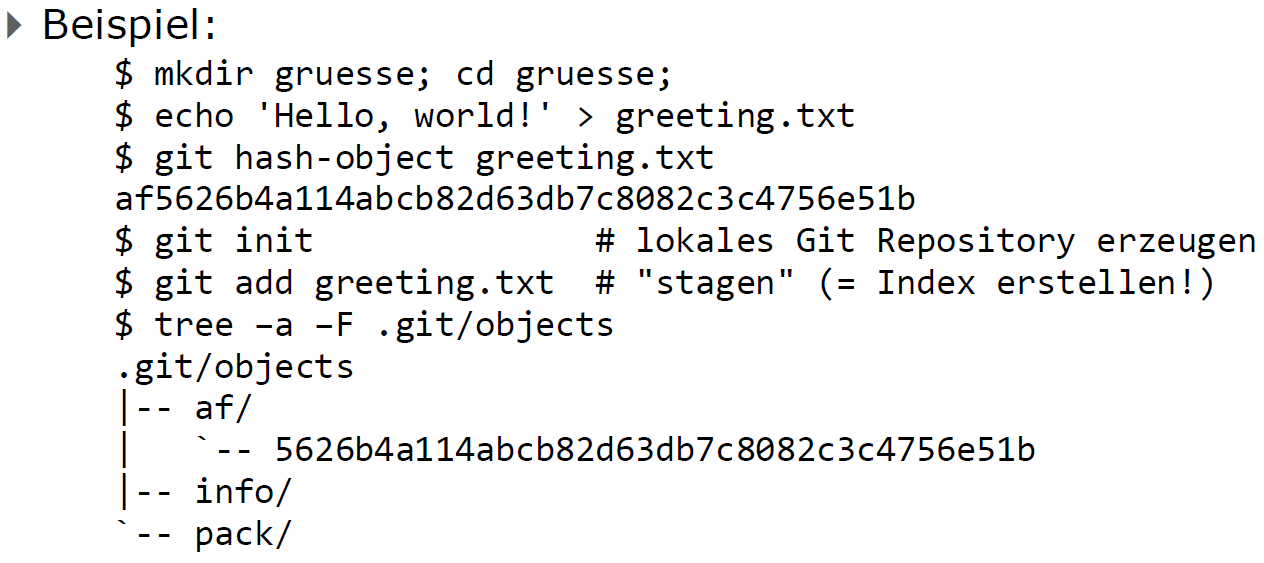
\includegraphics[width = 12cm]{images/gitobjekte}\\
	\begin{tabular}{|p{0.5\linewidth}|p{0.51\linewidth}|}
		\hline
		\begin{tabular}[c]{@{}l@{}}\textbf{blob} (\"{}binary large Object\"{})\\ -Inhalt einer Datei\\ -enthält \textit{keine} Zeiger auf andere Git-Objekte\end{tabular}   \newline  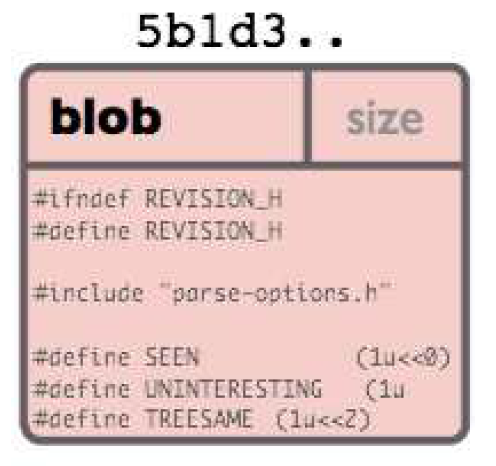
\includegraphics[width = 4cm]{images/blob}                             & \begin{tabular}[c]{@{}l@{}}\textbf{tree}\\ -enthält Zeiger auf blob-, oder tree-objekte\\ -enthält Referenzen über Git-Objekte, Ordner- \& Dateinamen\end{tabular} \newline 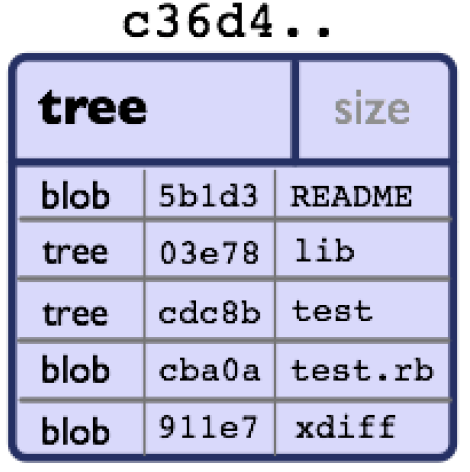
\includegraphics[width = 4cm]{images/tree} \\ \hline
		\begin{tabular}[c]{@{}l@{}}\textbf{commit}\\ -Startobjekt für einen Commit\\ -enthält Zeiger auf tree und vorgängiges Commit-Objekt\end{tabular} \newline 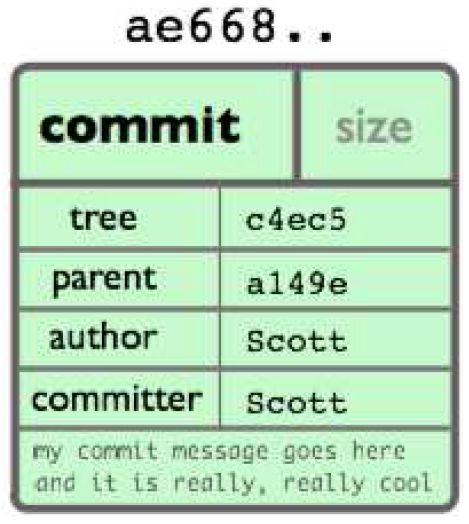
\includegraphics[width = 4cm]{images/commit}& \begin{tabular}[c]{@{}l@{}}\textbf{tag}\\ -Etikette mit Kommentar\\ -enthält Zeiger auf ein Commit-Objekt\end{tabular} \newline 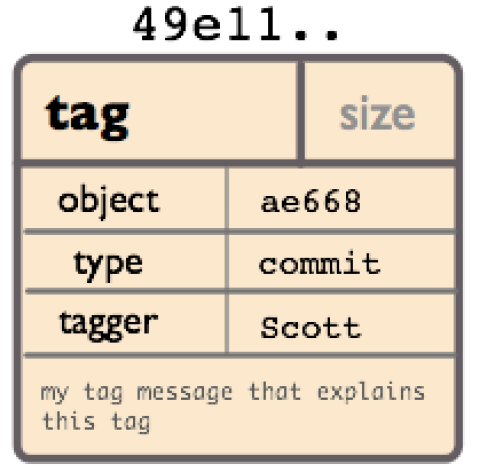
\includegraphics[width = 4cm]{images/tag}                                             \\ \hline
	\end{tabular}

\subsubsection{Git-Referenzen}
\begin{minipage}{10cm}
	\begin{itemize}
		\item Referenzen $=$ Zeiger (nur Zeigerwerte)
		\item Zeigen nur auf Git-Objekte
		\item Hashwert-Zeiger $\rightarrow$ zeigt auf Branches/Tags
		\item Symbolischer-Zeiger $\rightarrow$ zeigt auf Datei mit Namen eines anderen Zeigers
	\end{itemize}
\end{minipage}
\begin{minipage}{8cm}
	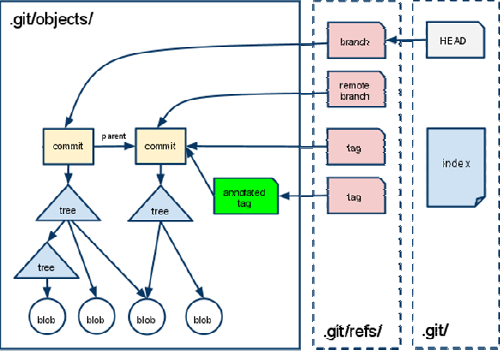
\includegraphics[width=8cm]{images/git-referenz.png}
\end{minipage}
\subsubsection{Bashprints}
\begin{multicols}{2}
	\begin{minipage}[l]{.40\textwidth}
		Files changed but not staged.\\    
		\textbf{\$ git status}\\
		On branch master\\
		Your branch is up-to-date with 'origin/master'.\\
		Changes not staged for commit:\\
		\quad (use "git add <file>..." to update what will be committed)\\
		\quad (use "git checkout -- <file>..." to discard changes in working directory)\\
		\\
		\qquad modified:\quad idiotenseite/IdiotenseiteInclude.tex\\
		\\
		no changes added to commit \newline (use \"{}git add\"{} and/or \"{}git commit -a\"{})\\
	\end{minipage}
	
	\begin{minipage}[r]{.40\textwidth}
		\textbf{\$ git log}\\
		commit 1b7ff854a491397087ff89689a535c275549e6ee\\
		Author: \quad Michel Gisler <Michel Gisler>\\
		Date:  \quad  Tue May 31 15:08:58 2016 +0200\\
		\\  
		\qquad Kleiner Ergänzungen und Anpassungen\\
	\end{minipage}
\end{multicols}
\clearpage
\pagebreak

\thispagestyle{empty}
\enlargethispage{3\baselineskip}
\subsubsection{Git Commands}
\vspace{-0.5cm}
\begin{longtable}{| p{.30\textwidth} | p{.70\textwidth} |}
	\hline 
	\textbf{Create}&
	\\ \hline
	
	git init <directory>&
	Create empty Git repo in specified directory.\newline
	Run with no arguments to initialize the current directory as a git repository.
	\\ \hline 
	
	git clone <repo>& 
	Clone repo located at <repo> onto local machine.\newline
	Original repo can be located on the local filesystem or on a remote machine
	\\ \hline  \hline
	
	\textbf{Local Changes}&
	\\ \hline 
	
	\hline 
	git status&
	List which files are staged, unstaged, and untracked  
	\\ \hline
	
	git diff& 
	Show unstaged changes between your index and working
	directory 
	\\ \hline 
	
	git diff HEAD&
	Show difference between working directory and last commit.
	\\ \hline
	
	git add <directory>&
	Stage all changes in <directory> for the next commit. Replace <directory>
	with a <file> to change a specific file or witch <.> to Stage all.
	\\ \hline 
	
	git commit -m " \" <message>"&
	Commit the staged snapshot, but instead of launching a text editor, use
	<message> as the commit message.
	\\ \hline
	
	git commit -a&
	Commit all local changes in tracked files.  
	\\ \hline 
	
	gitt commit --amend&
	Change the last commit. \textbf{Don‘t amend published commits!}
	\\ \hline \hline
	
    \textbf{Stash}&
    \\ \hline
    
    git stash&
    when you want to record the current state of the working directory 
    \\ \hline

    git stash list&
    Lists the modifications stashed away by this command
    \\ \hline
        
    git stash pop&
    Restore your stashed files
    \\ \hline \hline
        
    
	\textbf{Commit History}&  
	\\ \hline 
	
	\hline
	git log&
	Display the entire commit history using the default format.
	\\ \hline 
	
	git log -p <file>&
	Show changes over time for a specific file 
	\\ \hline
	
	git log --author="\"<pattern>"&
	Search for commits by a particular author. 
	\\ \hline
	
	git blame <file>& 
	Who changed what and when in <file>
	\\ \hline \hline
	
	\textbf{Branches and Tags}&  
	\\ \hline
	
	\hline
	git branch&
	List all of the branches in your repo. Add a <branch> argument to
	create a new branch with the name <branch>.
	\\ \hline 
	
	git branch <new-branch>&
	Create a new branch based
	on your current HEAD
	\\ \hline
	
	git branch -d <branch>&
	Delete a local branch
	\\ \hline   
	
	git branch -dr <remote/branch>&
	Delete a branch on the remote
	\\ \hline
	
	git checkout -b <branch>&
	Create and check out a new branch named <branch>. Drop the -b
	flag to checkout an existing branch.
	\\ \hline 
	
	git merge <branch>&
	Merge <branch> into the current branch.
	\\ \hline
	
	git tag <tag-name>&
	Mark the current commit with a tag (v1.0.1)
	\\ \hline  \hline
	
	\textbf{Update and Publish}&
	\\\hline 
	
	\hline
	git remote -v&
	List all currently configured remotes.
	\\ \hline 
	
	git remote add <name> <url>& 
	Add new remote repository, named <remote>
	\\ \hline 
	
	git fetch <remote>&  
	Download all changes from <remote>,
	but don‘t integrate into HEAD
	\\ \hline
	
	git pull <remote> <branch>&
	Download changes and directly merge/integrate into HEAD  
	\\ \hline 
	
	git push <remote> <branch>&
	Publish local changes on a remote
	\\ \hline \hline
	
	\textbf{ Merge and Rebase}&
	\\\hline 
	
	\hline
	git merge <branch>&
	Merge <branch> into your current HEAD
	\\ \hline 
	
	git rebase <branch>& 
	Rebase your current HEAD onto <branch>!\textbf{Don‘t rebase published commits!}
	\\ \hline 
	
	git rebase --abort&
	Abort a rebase
	\\ \hline 
	
	git mergetool& 
	Use your configured merge tool to solve conflicts
	\\ \hline \hline
	
	\textbf{Undo}&
	\\\hline 
	
	\hline
	git reset --hard HEAD&
	Discard all local changes in your working directory.
	\\ \hline  
	
	git checkout HEAD <file>&
	Discard local changes in a specific file
	\\ \hline   
	
	git revert <commit>&
	Revert a commit (by producing a new commit with contrary changes)
	\\ \hline    
	
	git reset <commit>&
	Move the current branch tip backward to <commit>, reset the staging area to match, but leave the working directory alone. 
	\\ \hline
\end{longtable}
\clearpage

\lstinputlisting[style=git]{source/Git/gitbefehle.cpp}
\lstinputlisting[style=git]{source/Git/gitbefehle1.cpp}
\pagebreak
\section{Qt}
\begin{minipage}{16cm}
	Qt (sprich cute = süss) ist eine plattformübergreifende Programmierungsapplikation für grafische \newline Benutzeroberflächen
    (GUI = Graphical User Interface).\\
	Qt wurde 1991 gegründet und gehörte der Firma Trolltech.
    Im Jahr 2008 übernahm Nokia die Firma Trolltech. Im Jahr 2014 wurde Qt als Open-Source-Projekt verwaltet. 
\end{minipage}
\begin{minipage}{1.5cm}
	
\includegraphics[width=1.5cm]{images/qt_logo.jpg}
\end{minipage}

\subsection{Grundlagen zu Qt}
\begin{minipage}{8cm}
	\begin{itemize}
		\item Qt C++ Klassenbibliothek stellt GUI-Elemente zur Verfügung
		\item Das GUI wird als C++ Sourcefile geschrieben
		\item Standardklasse QtGui und QtCore werden \newline automatisch inkludiert
		\item Alle Qt Widgets werden \textbf{auf dem Heap} erstellt
		\item Jedes Programm enthält eine Instanz von QApplication
		\item QApplication hält alles zusammen
	\end{itemize}
\end{minipage}
\begin{minipage}{10cm}
	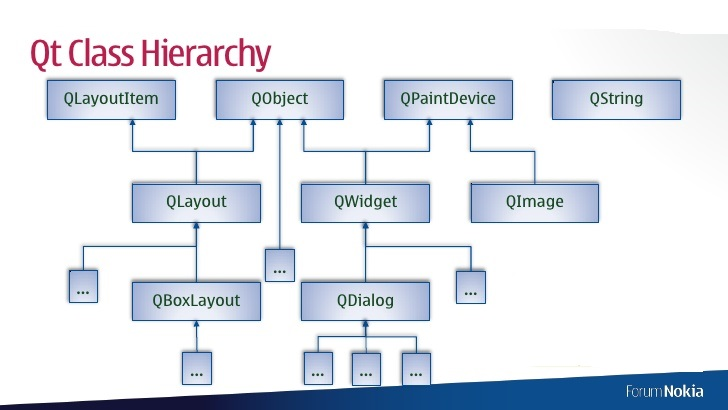
\includegraphics[width=10cm]{images/qt_classes.jpg}
\end{minipage}

\begin{multicols}{2}
	\subsubsection{QObject}
	\begin{itemize}
		\item QObject ist die \textcolor{blue}{Basisklasse des Qt-Modells}
		\item stellt das Memorymanagement (automatische delete) für alle abgeleitet Klassen von QObject zur \newline Verfügung. Es entstehen Objektbäume. 
		\item stellt die connect-Funktion zur Verfügung
		\item bearbeitet das Eventhandling
		\item hat keine visuelle Representation
	\end{itemize}
	
	\subsubsection{Qt Building: qmake}
	\begin{itemize}
		\item qmake Makefile-Generator
		\item macht aus plattformunabhängiem Projektfile (.pro) ein plattformspezifisches Projektfile. 
		\item die gewünschte Plattform wird qmake als Option \newline mitgegeben
		\item Bei Build-Problemen alle Dateien \textbf{ausser} .pro und Sourcefile löschen
	\end{itemize}
\end{multicols}

\subsubsection{Qt Konvention}
\begin{tabular}{|l|l|c|}
	\hline \textbf{Was}&\textbf{Beispiel} &\textbf{Konvention}
    \\ \hline   
    Qt-Modulname& "QtCore"&\textit{Qt}
    \\ \hline  
    Qt-Klassenname & "QString" &\textit{Q}
    \\ \hline   
    Qt-Variablen-,Funktionsname & "qTranslator, qDebug()"&\textit{q}
    \\ \hline   
    Qt-include & "\#include <QtGui>& \textit{ohne.h}
    \\ \hline
\end{tabular}

\subsection{QWidget (Widget = Window Gadget (\"{}Fenster Ding\"{})}
\begin{itemize}
	\item abgeleitet von QObject,  eine Instanz der Klasse stellt grafisches Element dar
	\item Diese Klasse hat viele Methoden um Aussehen, Grösse, Position etc. zu verändern
	\item mit show() wird das Widget angezeigt, mit hide() wird das Widget versteckt
	\item Jedes Widget wird einem \textit{"Parent-Widget"} (Eltern) zugewiesen, ein solches Widgets nennt man dann \textit{Child-Widgets}
	\item Durch die Parent-Child Funktion entsteht eine Verschachtelung
	\item Ein Widget \textbf{ohne} Parent ist ein Top-Level-Widget oder Window	
	\item Das \textit{"Parent-Widget"} übernimmt Verwaltungsfunktionen wie Memory-Management, \newline
    weiterleiten von Ereignisse an \textit{"Child-Widget}, anzeigen, verstecken von Widgets etc.
\end{itemize}

\begin{multicols}{3}
\subsubsection{Top-Level-Widget}
Die \textit{"Top-Level-Window"} sind Widgets welche auf der obersten \newline Hierarchiestufe liegen. Sie haben \newline keine \textit{"Parent-Widget"}.\newline
\textbf{Widgets} für \textit{"Top-Level-Window"}: 
\begin{itemize}
	\item \textcolor{blue}{QMainWindow} $\rightarrow$ Applikations-Window (Hauptfenster)
	\item \textcolor{blue}{QDialog} $\rightarrow$ Popup-Window für Abfragen ("Wirklich löschen?"), Hauptanwendung bleibt blockiert
	\item \textcolor{blue}{QWidget} $\rightarrow$ Einfaches Fenster
\end{itemize}

\subsubsection{Parent-Child-Widgets}
\begin{itemize}
	\item Jedes QObject kann \textbf{maximal ein} Eltern-QObject haben
	\item Jedes QObject kann beliebig \newline viele Kind-QObject haben
	\item Kind muss Eltern über sich \newline informieren
    \begin{itemize}
	\item Mit Konstruktor
    \subitem label->setParent(..)
    \item oder Layout Manager
    \end{itemize}
\end{itemize}

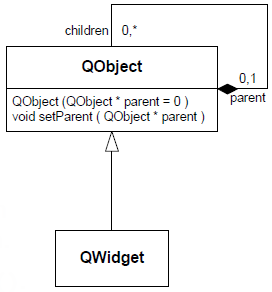
\includegraphics[width=5cm]{images/qt_parent_child.png}
\end{multicols}

\subsection{GUI-Programmierung}
Es gibt zwei grundlegende Aufgaben bei der GUI-Programmierung.\\
Das \textbf{Layout} legt Anordnung, Grösse  und Farbe fest.\\
Die \textbf{Interaktion} legt die Reaktion des Programmes auf eine Eingabe fest. \\

\subsection{Layout}
Es gibt \textbf{drei Varianten} wie Widgets innerhalb eines Widget angeordnet werden können: \newline
\textcolor{blue}{
    \begin{itemize}
        \item Absolute Positionierung
        \item Layout Manager
        \item GUI-Designer (Qt Designer)
    \end{itemize}
}

\subsubsection{Absolute Positionierung}
Mittels Methoden:
\begin{multicols}{2}
    \begin{minipage}{1.08\linewidth}
        \lstinputlisting[style=c++qt,linewidth=\linewidth]{source/Qt/methoden.cpp}
        \subsubsection{Layout Manager} %TODO Layout?
        \begin{tabular}{|l|l|}
            \hline \textbf{Klasse} & \textbf{Ort}\\
            \hline QVBoxLayout & Elemente vertikal\\
            \hline QHBoxLayout & Elemente horizontal\\
            \hline QGridLayout & zweidimensionales Gitter\\
            \hline QFormLayout & Elemente zeilenweise\\
            \hline QStackedLayout & aufeinandergelegt Widgets\\
            \hline
        \end{tabular}
       \end{minipage}	
		
	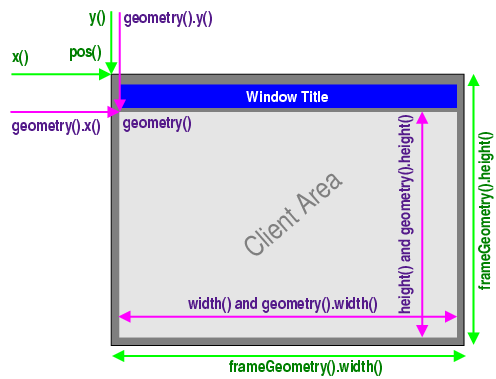
\includegraphics[width=0.8\linewidth]{images/geometry.png}
\end{multicols}
	
\subsubsection{GUI-Designer / Qt Designer}	
	Im Qt Designer mittels Drag-Drop können die Elemente angeordnet werden, anschliessend Umwandlung in Code. 	

\subsection{Interaktion}
In Qt werden die Eingaben als SIGNALS bezeichnet und die Ausgaben als SLOTS. Mittels der Funktion connect() werden die beiden miteinander verknüpft.\\
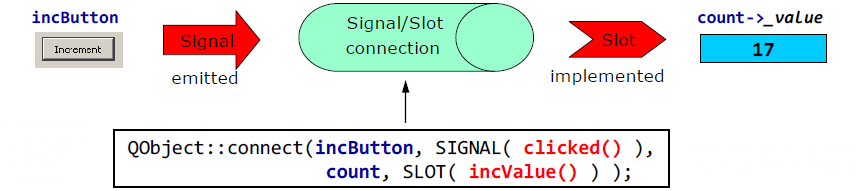
\includegraphics[width=15cm]{images/connect.png}

\begin{multicols}{3}
\subsubsection{SIGNALS}
\begin{itemize}
	\item nur deklariert, nie definiert
	\item kein Zugriffsrecht vergeben
	\item Rückgabetyp immer void
\end{itemize}

\subsubsection{SLOTS}
\begin{itemize}
	\item deklariert und definiert
	\item oftmals Memberfunktion, auch normal abrufbar
	\item Zugriffsrechte
\end{itemize}

\subsubsection{connect}
\begin{itemize}
	\item Verbindungsfunktion zwischen Input und Output
	\item ein Signal zu mehreren Slots
	\item mehrere Signale zu einem Slot
\end{itemize}
\end{multicols}

\vspace{0.5pt}
\textbf{Beispiele connect-Funktion}
\lstinputlisting[style=c++qt]{source/Qt/connect.cpp}

\subsection{Zeichnen und Malen}
\begin{multicols}{2}
	\subsubsection{QPainter}
	Der Maler mit Mal-\& Zeichenwerkzeugen.\\
	
	\begin{tabular}{|l|l|}
		\hline \textbf{Klasse} & \textbf{Werkzeug}\\
		\hline QPen & Zeichenstift\\
		\hline QBrush & Pinsel\\
		\hline QFont & Schriftart\\
		\hline draw & Formen malen\\
		\hline
	\end{tabular}
	
	\subsubsection{QPaintDevice}
	Oberfläche wo darauf gezeichnet \& gemalt werden kann
	QPainter-Objekte zeigen auf QPaintDevice-Objekte. QPaintDevice ist eine abstrakte Basisklasse welche nicht von QObject abgeleitet ist und daher \textbf{kein automatisches delete.}\\

\end{multicols}

\subsubsection{Vorgehen}
\lstinputlisting[style=c++qt]{source/Qt/qpainter.cpp}
\pagebreak
\section{Beispiele}

\subsection{CppUnit}
\lstinputlisting[style=cppunit]{source/CppUnit/AuthorTest.cpp}
\newpage
\lstinputlisting[style=cppunit]{source/CppUnit/testdatum.cpp}

\subsection{Doxygen}
\begin{tabular}{p{0.5\linewidth} p{0.5\linewidth}}
	\textbf{Eclipse Einstellungen}\newline
	\tabbild[width=9cm]{images/doxygen_advanced.png} &
    \textbf{Eclipse-Plugin} \newline
    \tabbild[width=9cm]{images/doxygen_basic.png}
\end{tabular}
\newpage
\begin{multicols}{2}
	\lstinputlisting[style=cdoxy,linewidth=11cm]{source/Doxygen/doxygenbsp.c}	
	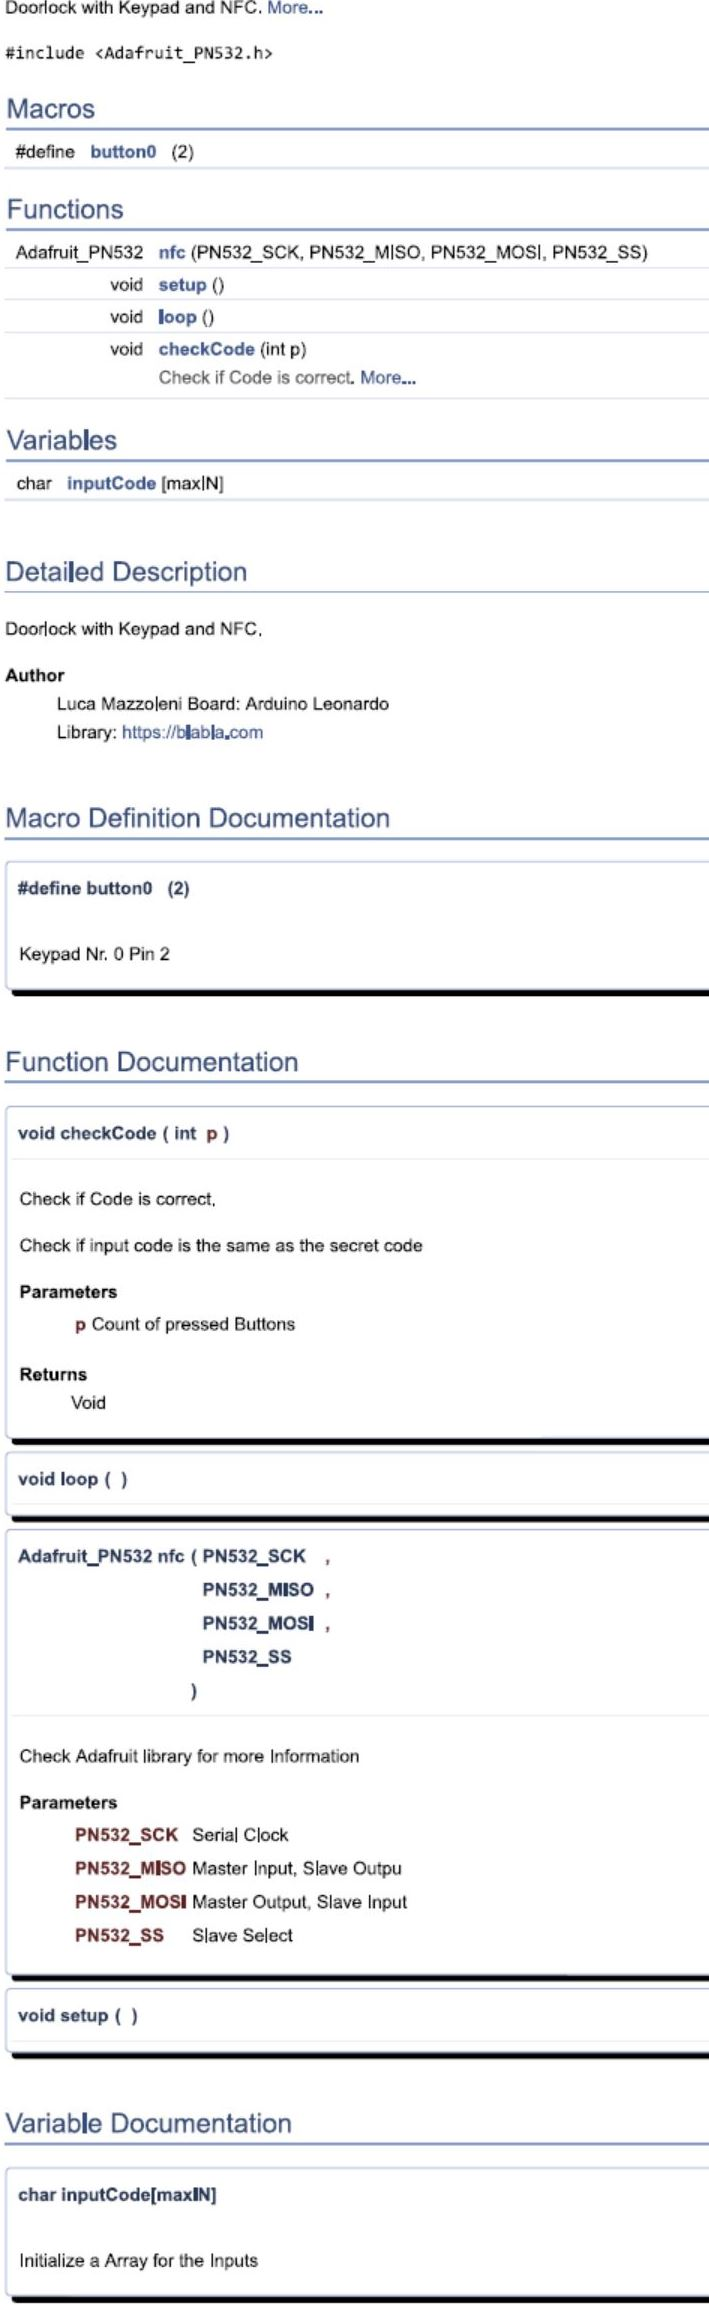
\includegraphics[width=8cm]{images/html.JPG}
\end{multicols}	
\pagebreak
%=================================

\subsection{Qt}
\subsubsection{HTML-Tags}
\lstinputlisting[style=c++qt]{source/Qt/html.cpp}
\begin{longtable}{| p{.15\textwidth} | p{.30\textwidth} | p{.45\textwidth}|}
	\hline \textbf{Tag} & \textbf{Description} & \textbf{Comment}\\
	\hline a& Anchor or link& \\
	\hline address & Address &\\
	\hline b& Bold & \textbf{Fett}\\
	\hline big & Larger font&\\
	\hline blockquote & Indented paragraph&\\
	\hline body & Document body &\\
	\hline br & Line break &\\
	\hline center & Centered paragraph&\\
	\hline cite & Inline citation & Same as i\\
	\hline code & Code& Same as tt\\
	\hline dd & Definition data & \\
	\hline dfn & Definition & \\
	\hline div& Document divison&\\
	\hline em& Emphasized& \emph{Same as i}\\
	\hline font& Font size, family, color& Support size, face, color (Qt::green) attributes\\
	\hline h1 & Level 1 heading& Titel 1. Ordnung\\
	\hline h2 & Level 2 heading& Titel 2. Ordnung\\
	\hline h3 & Level 3 heading& Titel 3. Ordnung\\
	\hline h4 & Level 4 heading& Titel 4. Ordnung\\
	\hline h5 & Level 5 heading& Titel 5. Ordnung\\
	\hline h6 & Level 6 heading& Titel 6. Ordnung\\
	\hline head & Document header&\\
	\hline hr & Horizontal line&\\
	\hline html & HTML document&\\
	\hline i & italic& \textit{kursiv}\\
	\hline img&image& Support src, source, width, height attributes\\
	\hline kbd& User entered text&\\
	\hline meta & Meta-information& Text in Metacode in HTML\\
	\hline li & List-Item& Jeder einzelne Punkt muss umschlossen werden.\\
	\hline nobr & Non-breakable text&\\
	\hline ol & Ordered list& \\
	\hline p & paragraph&\\
	\hline pre & preformated text& \\
	\hline qt & Qt richt-text document& Synonym für HTML\\
	\hline s& Strikethrough&\\
	\hline samp & Sample Code&\\
	\hline small & Small font &{\scriptsize kleine Schrift}\\
	\hline strong & Strong & \textbf{same as b}\\
	\hline style & Style sheet & Allows styling information to be included with rich text\\
	\hline title & Document row & \\
	\hline u & underlined & \\
	\hline var & Variable & Same as i\\
	\hline
\end{longtable}
\clearpage
\newpage
\subsubsection{QWidgets}
\begin{tabular}{c c}
	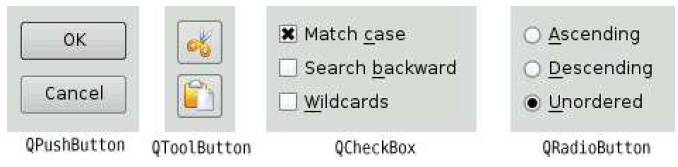
\includegraphics[width=9cm]{images/button_1.png}&
    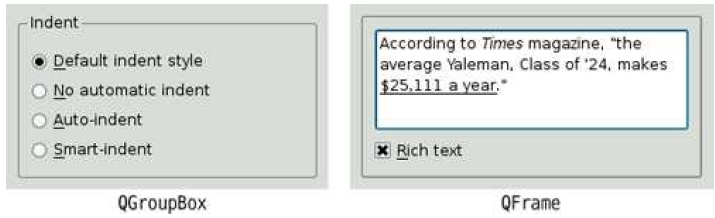
\includegraphics[width=9cm]{images/button_2.png}\\
	\includegraphics[width=9cm]{images/button_3.png}&
    \includegraphics[width=9cm]{images/button_7.png}\\
	\includegraphics[width=9cm]{images/button_4.png}&
	\includegraphics[width=9cm]{images/button_5.png}\\
	\includegraphics[width=9cm]{images/button_6.png}&
	\includegraphics[width=9cm]{images/button_8.png}\\
\end{tabular}
\subsubsection{QBrush}
\includegraphics[width=9cm]{images/brush.png}

%\begin{multicols}{2}
    \begin{minipage}{0.6\linewidth}
        \subsubsection{QPainter draw-Methoden}
        \includegraphics[width=\linewidth]{images/draw_1.png}\newline
        \includegraphics[width=\linewidth]{images/draw_2.png}
    \end{minipage}
    
    \begin{minipage}{0.6\linewidth}
        \subsubsection{QPen}
        \includegraphics[width=\linewidth]{images/pen_1.png}\newline \includegraphics[width=\linewidth]{images/pen_2.png}\newline   
    \end{minipage}
%\end{multicols}
\clearpage
\subsubsection{SpezUeb}
\begin{longtable}{l l} %Error but works.. IDC
    \textbf{GridLayout}&\\
    \lstinputlisting[style=c++qt,linewidth=12cm]{source/Qt/SpezUeb1.cpp}&
    \hspace{-2cm}\includegraphics{images/qtSpezUeb1.jpg}
    \\&\\
    \lstinputlisting[style=c++qt,linewidth=12cm]{source/Qt/GridLayout.cpp}&
    \hspace{-2cm}\includegraphics{images/GridLayout.jpg}  
    \\ 
    \\&\\ 
    \textbf{Quiz}&\\
    \lstinputlisting[style=c++qt,linewidth=12cm]{source/Qt/SpezUeb2.cpp}&
    \includegraphics{images/qtSpezUeb2.jpg}
    \\
    \textbf{Signal and Slots}&\\
    \lstinputlisting[style=c++qt,linewidth=12cm]{source/Qt/SpezUeb3.cpp}&
    \hspace{-2cm}\includegraphics{images/qtSpezUeb3.jpg} 
\end{longtable}
%TODO JPG smaller or Print it Standalone A3
%\newpage 
%\includegraphics[angle=90,origin=c,width=\linewidth]{images/qt3classchart}
%\newpage
%=================================================
\clearpage
\subsubsection{Hello World}
\lstinputlisting[style=c++qt]{source/Qt/hello_world.cpp}

\subsubsection{Temperaturwidget}
\textbf{main.cpp}
\\
\begin{multicols}{2}
\lstinputlisting[style=c++qt]{source/Qt/main.cpp}

\includegraphics[width=\linewidth]{images/temperaturwidget}
\end{multicols}

\textbf{temperaturwidget.h}
\\
\lstinputlisting[style=c++qt]{source/Qt/temperaturwidget.h}
\newpage
\textbf{temperaturwidget.cpp}
\lstinputlisting[style=c++qt]{source/Qt/temperaturwidget.cpp}

\subsubsection{Counter-implementation}
\begin{multicols}{2}
    \begin{minipage}{\linewidth}
       \textbf{Implementation mit Klassen}\newline
       \textbf{main (Klassen).cpp}
       \lstinputlisting[style=c++qt]{source/Qt/countermain2.cpp}
       \textbf{mydialog.h}
       \lstinputlisting[style=c++qt]{source/Qt/mydialog.h}
       \textbf{mydialog.cpp}
       \lstinputlisting[style=c++qt]{source/Qt/mydialog.cpp}
    \end{minipage}

    \begin{minipage}{\linewidth}
        \includegraphics[width=0.5\linewidth]{images/count1}\newline
        \textbf{Implementation \"{}nur\"{} im main.cpp}
        \lstinputlisting[style=c++qt]{source/Qt/countermain1.cpp}
    \end{minipage}
\end{multicols}
\clearpage
\textbf{counter.h}\newline
\lstinputlisting[style=c++qt]{source/Qt/counter.h}
\textbf{counter.cpp}\newline
\lstinputlisting[style=c++qt]{source/Qt/counter.cpp}
%=================================================
\clearpage
\textbf{CircleButton}
\begin{multicols}{2}
    \lstinputlisting[style=c++qt]{source/Qt/CircleButton/main.cpp}
    
\begin{minipage}{0.8\linewidth}
    \includegraphics[width=0.5\linewidth]{images/circlebutton1}\includegraphics[width=0.5\linewidth]{images/circlebutton2}
    \newline
    \newline
\end{minipage}
\end{multicols}
\lstinputlisting[style=c++qt]{source/Qt/CircleButton/Demo1CircleButton.h}
\lstinputlisting[style=c++qt]{source/Qt/CircleButton/Demo1CircleButton.cpp}
\clearpage
\lstinputlisting[style=c++qt]{source/Qt/CircleButton/CircleButton.h}
\lstinputlisting[style=c++qt]{source/Qt/CircleButton/CircleButton.cpp}




\pagebreak
\null\pagebreak\null\pagebreak %Um bei booklet auf der lezten Seite zu sein: S.40 +k x 4
\section*{Glossar}
\begin{tabular}{ll}
   API  & Application Program Interface \\ 
   CVCS & Central Version Control System \\ 
   DMS  & Document Management System \\ 
   DVCS & Distributed Version Control System \\ 
   FIT  & Framework for Integrated Test\\
   GUI  & Graphical User Interface \\ 
   LVCS & Local Version Control System\\ 
   moc  & Meta Object Compiler\\
   OOA  & Objekt Orientierte Analyse\\
   OOD  & Objekt Orientiertes Design\\
   OOI  & Objekt Orientierte Implementation\\
   PAP  & Projekt Ablauf Plan\\ 
   PC   & Projektleiter\\ 
   PSP  & Projekt Struktur Plan\\ 
   RUP  & Rational Unified Prcess\\
   SHA  & Secure Hash Algorithmus\\ 
   SUT  & System Under Test\\
   UML  & Unified Modeling Language\\
   VCS  & Version Control System\\ 
   XP   & Xtreme Programming \\ 
\end{tabular}  
\end{document}